% ---------------------------------------------------------------
% ---------------------------------------------------------------
% Modelo de Trabalho Acadêmico utilizando classe repUERJ para
% elaboração de teses, dissertação e trabalhos monográficos em
% geral.
%
% Este arquivo está editado na codificação de caracteres UTF-8.
%
% As referencia estão baseadas no modelo bibtex e citação em
% autor-data
%
% Este modelo foi criado por 
% 	Dr. Luís Fernando de Oliveira
% 	Professor Adjunto do Dep. de Física Aplicada e Termodinâmica
% 	Instituto de Física Armando Dias Tavares
% 	Universidade do Estado do Rio de Janeiro - UERJ
%
% A classe repUERJ.cls foi criada a partir do código original 
% disponibilizado pelo grupo CódigoLivre (coordenado por
% Gerald Weber). Foram feitas adequações para implementação das 
% normas de elaboração de teses e dissertações da UERJ.
%
% Os estilos repUERJformat.sty codificam os elementos
% pré-textuais e pós-textuais.
%
% O estilo repUERJpseudocode.sty codifica a elaboração de
% algoritmos utilizando um glossário desenvolvido por mim
% (Luís Fernando), o mesmo usado em meu curso de Física
% Computacional.
%
% Todo este material está disponível também no meu site
%      http://sites.google.com/site/deoliveiralf
%
% As normas da UERJ para elaboração de teses e dissertações 
% pode ser obtidas no documento disponível no site
%      http://www.bdtd.uerj.br/roteiro_uerj_web.pdf
%
% Agradecimentos ao NPROTEC/Rede Sirius/UERJ e à Biblioteca
% Setorial da Física.
% ---------------------------------------------------------------
% ---------------------------------------------------------------
%
% Adaptado para o Departamento de Eng. de Sistemas e Computação pelo
% professor João Araujo
\documentclass[a4paper,12pt,oneside,onecolumn,final,fleqn]{repUERJ}
% ---
% Pacotes fundamentais 
% ---
\usepackage[brazil]{babel}  % adequação para o português Brasil
\usepackage[utf8]{inputenc} % Determina a codificação utilizada
% (conversão automática dos acentos)
\usepackage{makeidx}        % Cria o índice
\usepackage{hyperref}       % Controla a formação do índice
\usepackage{indentfirst}    % Indenta o primeiro paragrafo de
% cada seção.
\usepackage{graphicx}       % Inclusão de gráficos
\usepackage{subfig}
\usepackage{multirow}
\usepackage{amsmath,amssymb}  % pacotes matemáticos
\usepackage[alf]{abntex2cite} % pacote para citacoes
\usepackage[font=default,frame=no]{repUERJformat} % pacote para as 
% normas da UERJ
% ---
% pacote auxiliar para elaboração de pseudocódigos
% este pacote pode ser retirado caso nao se planeje
% elaborar pseudocódigos
% ---
\usepackage[dots=yes]{repUERJpseudocode}
\usepackage{listings}
\lstset{language=XML, 
	keywordstyle=\color{blue},
	basicstyle=\small,
	showstringspaces=false,
	xleftmargin=0pt,
	extendedchars=true,
	inputencoding=utf8,
	frame=none,
	breaklines=true,
	emph={True,False},
	texcl=true,
	literate={á}{{\'a}}1 {à}{{\`a}}1 {ã}{{\~a}}1 {â}{{\^a}}1 {é}{{\'e}}1 {í}{{\'i}}1 {ó}{{\'o}}1 {ú}{{\'u}}1 
	{ê}{{\^e}}1 {é}{{\'e}}1 {ô}{{\^o}}1 {õ}{{\~o}}1 {ç}{{\c{c}}}1 {º}{${^\circ}$}1,, 
	commentstyle=\color{red},
	tabsize=2,
	stringstyle=\color{red},
	columns = fixed
} 

\usepackage[maxfloats=25]{morefloats}
\usepackage{array}
\usepackage{multirow}
\setlength\extrarowheight{2pt}

% ***************************************************************
% Informações de autoria e institucionais
% ***************************************************************

%----------------------------------------------------------------
% Imagens pretextuais (precisam estar no mesmo diretório deste arquivo .tex)
%----------------------------------------------------------------

\logo{logo_uerj_cinza.png}
\marcadagua{marcadagua_uerj_cinza.png}{1}{160}{255}

%----------------------------------------------------------------
% Informações da instituição
%----------------------------------------------------------------

\instituicao{Universidade do Estado do Rio de Janeiro}
{Centro de Tecnologia e Ciências}  
{Faculdade de Engenharia}
{Departamento de Sistemas e Computação} 

%----------------------------------------------------------------
% Informações da autoria do documento
%----------------------------------------------------------------

% \oautor{Nóme}{Sóbrenome}
%       {Iniciais do nome} % iniciais do nome

\autor{Matheus}{Vargas}
{M.V.} % iniciais do nome

\titulo{Adaptação do Software E-foto para Atendimento aos Requisitos de Pacotes Debian-gis}
\title{Adaptation of e-foto software to meet the requirements of debian-gis packages}

% se não for usar a quarta palavra chave, deixar o campo vazio: {}
\palavraschaves{Primeira palavra-chave}
{Segunda palavra-chave}
{Terceira palavra-chave}
{Quarta palavra-chave (opcional) ou vazio}

\keywords{First keyword}
{Second keyword}
{Third keyword}
{Fourth keyword or empty}

\orientador{Prof. Dr.} 
{João}{Araujo Ribeiro} 
{Unidade -- UERJ} 


%----------------------------------------------------------------
% Grau pretendido (Doutor, Mestre, Bacharel, Licenciado) e Curso
%----------------------------------------------------------------

\grau{Engenheiro} % Doutor, Mestre, Bacharel, Licenciado
\curso{Graduação}
%\areadeconcentracao{linha de pesquisa} % opcional

%----------------------------------------------------------------
% Informações adicionais (local, data e paginas)
%----------------------------------------------------------------

\local{Rio de Janeiro} 
\data{dd}{mês}{2021} 

% ***************************************************************
% Configurações de aparência do PDF final
% ***************************************************************

% alterando o aspecto da cor azul
%\definecolor{blue}{RGB}{41,5,195}
%\definecolor{apricot}{RGB}{251,206,177}

% informações do PDF
\hypersetup{
	unicode=false,
	pdftitle={\UERJtitulo},
	pdfauthor={\UERJautor},
	pdfsubject={\UERJpreambulo},
	pdfkeywords={PALAVRAS-CHAVES:}{ \chaveA}{ \chaveB}{ \chaveC}{ \chaveD},
	pdfproducer={\packagename}, % producer of the document
	colorlinks=true,   % false: boxed links; true: colored links
	linkcolor=black,   % color of internal links blue
	citecolor=black,   % color of links to bibliography blue
	filecolor=black,   % color of file links magenta
	urlcolor=black,
	bookmarksdepth=4,
	%   backref=true,
	%   pagebackref=true,
	%   bookmarks=true,
}

% ***************************************************************
% Índice remissivo
% ***************************************************************
%
\makeindex % compila o índice; se não for usar, comentar
%
% ***************************************************************
% Fim do preâmbulo
% ***************************************************************

%/\/\/\/\/\/\/\/\/\/\/\/\/\/\/\/\/\/\/\/\/\/\/\/\/\/\/\/\/\/
\begin{document}
	%/\/\/\/\/\/\/\/\/\/\/\/\/\/\/\/\/\/\/\/\/\/\/\/\/\/\/\/\/\/
	
	%XXXXXXXXXXXXXXXXXXXXXXXXXXXXXXXXXXXXXXXXXXXXXXXXXXXXXXXXXXXXXXXX
	% ELEMENTOS PRE-TEXTUAIS
	%XXXXXXXXXXXXXXXXXXXXXXXXXXXXXXXXXXXXXXXXXXXXXXXXXXXXXXXXXXXXXXXX
	\frontmatter % inicia a área dos elementos pré-textuais
	%XXXXXXXXXXXXXXXXXXXXXXXXXXXXXXXXXXXXXXXXXXXXXXXXXXXXXXXXXXXXXXXX
	
	% ----------------------------------------------------------
	% Capa e a folha de rosto
	% ----------------------------------------------------------
	%
	\capa
	\folhaderosto
	%
	% ----------------------------------------------------------
	% Inserir a ficha catalográfica
	% ----------------------------------------------------------
	% ---
	% A biblioteca deverá providenciar a ficha catalográfica. 
	% Salve a ficha no formato PDF. Use o nome do arquivo PDF 
	% como argumento do comando. 
	% Exemplo: ficha catalográfica no arquivo 'ficha.pdf'
	%     \fichacatalografica{ficha.pdf}
	%
	% Enquanto não possuir a ficha catalográfica, use o comando sem
	% argumentos.
	% ---
	%
	\fichacatalografica{}
	%
	% ----------------------------------------------------------
	% Folha de aprovação
	% ----------------------------------------------------------
	%
	\begin{folhadeaprovacao}
		\assinatura{Cargo Título Nome Completo}
		{Unidade -- Instituição}
		\assinatura{Cargo Título Nome Completo}
		{Unidade -- Instituição}
		\assinatura{Cargo Título Nome Completo}
		{Unidade -- Instituição}
		\assinatura{Cargo Título Nome Completo}
		{\UERJunidade \UERJunidadenome\ -- UERJ}
	\end{folhadeaprovacao}
	%
	% ----------------------------------------------------------
	% Dedicatória
	% ----------------------------------------------------------
	%
	\pretextualchapter{Dedicatória}
	\vfill
	Texto da dedicatória (opcional).
	%
	% ----------------------------------------------------------
	% Agradecimentos
	% ----------------------------------------------------------
	%
	\pretextualchapter{Agradecimentos}
	
	Texto de agradecimento (opcional).
	%
	% ----------------------------------------------------------
	% Epigrafe (opcional)
	% ----------------------------------------------------------
	%
	\pretextualchapter{}
	\vfill
	\begin{flushright}
		(opcional)\\
		Pensamento, reflexão\\    
		\textit{autor}
	\end{flushright}
	%
	% ----------------------------------------------------------
	% RESUMO
	% ----------------------------------------------------------
	%
	\pretextualchapter{Resumo}
	\referencia % linha em branco depois
	
	Texto do resumo em português.
	~\\
	
	\imprimirchaves % linha em branco antes
	%
	% ----------------------------------------------------------
	% Abstract
	% ----------------------------------------------------------
	%
	\pretextualchapter{Abstract}
	\reference % linha em branco depois
	
	Texto do resumo em inglês.
	~\\
	
	\printkeys % linha em branco antes
	%
	% ----------------------------------------------------------
	% Listas de ilustrações e tabelas
	% ----------------------------------------------------------
	%
	\listadefiguras
	\listadegraficos
	\listadequadros
	\listadetabelas
	%
	% ----------------------------------------------------------
	% Outras listas
	% ----------------------------------------------------------
	%
	\listadealgoritmos % opcional
	%
	% ----------------------------------------------------------
	% Lista de abreviaturas e siglas (opcional)
	% ----------------------------------------------------------
	%
	\pretextualchapter{Lista de abreviaturas e siglas}
	\abreviatura{sigla 1}{por extenso}
	\abreviatura{sigla 2}{por extenso}
	\abreviatura{sigla 3}{por extenso}
	%
	% ----------------------------------------------------------
	% Lista de simbolos (opcional)
	% ----------------------------------------------------------
	%
	\pretextualchapter{Lista de símbolos}
	\simbolo{$simbolo 1$}{significado e/ou valor}
	\simbolo{$simbolo 2$}{significado e/ou valor}
	\simbolo{$simbolo 3$}{significado e/ou valor}
	%
	% ----------------------------------------------------------
	% Sumario
	% ----------------------------------------------------------
	%
	\sumario
	%
	%XXXXXXXXXXXXXXXXXXXXXXXXXXXXXXXXXXXXXXXXXXXXXXXXXXXXXXXXXXXXXXXX
	% ELEMENTOS TEXTUAIS
	%XXXXXXXXXXXXXXXXXXXXXXXXXXXXXXXXXXXXXXXXXXXXXXXXXXXXXXXXXXXXXXXX
	\mainmatter % inicia a área de desenvolvimento do conteúdo
	%XXXXXXXXXXXXXXXXXXXXXXXXXXXXXXXXXXXXXXXXXXXXXXXXXXXXXXXXXXXXXXXX
	
	
	
	%================================================================
\chapter*{Introdução}
%================================================================

\begin{epigrafeonline}
\hfill Texto da epígrafe \textit{in locu}.\\
\hspace*{\fill}\textit{Autor}\\
\end{epigrafeonline}
% explique aqui a importância de seu projeto
Texto da introdução.
	%================================================================
\chapter{O programa E-foto}
%================================================================

Nesse capítulo será apresentado o software E-foto, suas funcionalidades e o que deve ser feito para sua obtenção e instalação. Sendo explicado quais pacotes serão necessários para o funcionamento do programa após a realização do seu download.

\section{O que é o E-foto}
\subsection{O que é e qual o objetivo do E-foto}
De acordo com o site oficial\footnote{\url{http://www.efoto.eng.uerj.br/about-e-foto}}, o E-foto é um software livre para fotogrametria digital que é desenvolvido pelo laboratório de fotogrametria da Universidade do Estado do Rio de Janeiro desde 2004 e tem como objetivo, além da criação de um software inteiramente funcional (uma estação fotogramétrica gratuita), levar aos alunos o conhecimento de forma gratuita sobre fotogrametria digital, sendo de forma didática ou até mesmo na prática por meio de acesso ao código, uso da plataforma e até criação de novos módulos para o software.

\subsection{O que é a fotogrametria}
A fotogrametria remete etimologicamente à ideia da realização de medidas em imagens, e tem como objetivo geral a recriação de parte de um espaço tridimensional a partir de imagens bidimensionais obtidas sem contado entre o sensor e o alvo fotografado. A fotogrametria é classificada de acordo com a evolução dos métodos de obtenção e de análise das imagens, cuja realização deixou de ser analógica e se tornou digital em tempos atuais, aumentando a precisão e a velocidade, e deixando de lado o trabalho mais artesanal e demorado.
Segundo a \textit{American Society for Photogrammetry and Remote Sensing} (ASP, 1980):

\begin{quote}
	``A fotogrametria é a arte, ciência, e tecnologia de obtenção de informações confiáveis sobre os objetos físicos e o meio ambiente por meio de processos de gravação, medição e interpretação de imagens fotográficas e padrões da energia eletromagnética radiante e outros fenômenos.''
\end{quote}

\subsection{Classificações da fotogrametria}
Usando como referência o  livro \textbf{Fotogrametria Digital}, escrito por Luiz Coelho e Jorge Nunes Brito \cite{bib:livrofotogrametria}, publicado pela Editora da Universidade do Estado do Rio de Janeiro, podemos dizer que as classificações da fotogrametria são feitas de maneira histórica. Assim, a \textbf{fotogrametria pioneira} (1840-1900) se deu alguns anos após a invenção da fotografia e com a ideia de usá-la para auxílio na topografia, mas sem grandes resultados, sua utilização começou mesmo a ser difundida em 1851 para documentação de edifícios históricos, sendo criados os seus primeiros métodos de utilização, mas somente com avanços na tecnologia aérea a fotogrametria pôde realmente ser impulsionada e a dificuldade na obtenção de imagens aéreas foi reduzida. 

%fazer gráfico com linha do tempo das classificações da fotogrametria

A \textbf{fotogrametria analógica} (1901-1950) se deu após a primeira revolução da fotogrametria, que ocorre com a invenção do aparelho \textit{estereocomparador} que colocava aparelhos óptico mecânicos no lugar de inúmeros cálculos matemáticos, facilitando a vida dos usuários. Em 1911 foi aumentado o uso de retificadores analógicos devido à criação de um método funcional de retificação de imagens que tornou usual a utilização das fotografias para mapear extensas superfícies. A Alemanha e a Suíça tinham aparelhos que tornavam possíveis a criação de cartas topográficas de alta precisão. Esse avanço na tecnologia da fotogrametria fez com o trabalho se tornasse cada vez mais especializado, assim passou a ter necessidade de um profissional de conhecimento técnico para a realização do mesmo. Paralelamente a esse avanço ocorreram também mais fatos que ajudaram no avanço da fotogrametria em geral, o processo de foto triangulação analógica facilitou o trabalho externo, as câmaras métricas que realizavam impressões de imagens relevantes quanto às coordenadas, o que fez aumentar a precisão das medidas realizadas.

A partir da evolução da tecnologia computacional, grande parte do trabalho manual e mecânico foram substituídos por tarefas feitas diretas no computador dando início a era da \textbf{fotogrametria analítica} (1951-1990). Com o auxílio da computação os cálculos em cima das imagens eram feitos pelos computadores e passou a ter a possibilidade da utilização de conjunto de imagens para serem medidas simultaneamente assim como um estudo mais completo da propagação de erros, passou a ser permitido também a utilização de câmeras não-métricas.

Com o avanço tecnológico ocorreram mudanças bem significativas no quesito de obtenção de imagens, uma vez que com a criação das câmeras digitais ou até mesmo com a utilização de um escâner se pôde obter imagens digitais. Com avanços da computação os computadores passaram a processar essas imagens, com isso surgiu a era da \textbf{fotogrametria digital} (1990-atualmente). Para o processo foram criadas estações com aparelhos específicos para a fotogrametria, as chamadas estações fotogramétricas digitais, nas quais todo o processo é feito por meio de computadores, desde a sua entrada (fotos digitais ou analógicas digitalizadas) até a sua saída (dados digitais compatíveis com programas existentes).

\subsection{Obtenção de imagens fotogramétricas digitais}
Podemos obter uma imagem fotogramétrica digital de duas maneiras: por meio de escâneres (digitalização de imagens obtidas analogicamente) e por meio de câmeras fotogramétricas digitais (maneira mais direta). Com a utilização dos escâneres normalmente é possível obter a melhor configuração para a digitalização desejada, mas mesmo com essa configuração, existe a ocorrência de perda de alguma informação durante o processo de digitalização, posto que os dispositivos não possuem capacidade de digitalizar toda a complexidade da imagem. %Por que?

Essa responsabilidade de configurar os escâneres e seus respectivos programas para que a perda seja menor possível de maneira que a imagem ainda possa ser utilizada e mantendo a integridade da imagem original é humana, do profissional da área fotogramétrica. No caso do uso das câmeras fotogramétricas digitais ainda existe muita limitação para seu uso, pois possuem um preço muito elevado. %Isso ainda se mantém? Pesquisar 
Ainda podem ocorrer problemas na obtenção das imagens devido ao formato das lentes das câmeras, o que também deve ser tratado para manter a integridade de uma imagem fotogramétrica digital.

\subsection{Importância e os problemas da fotogrametria digital}
A importância da fotogrametria digital é justamente manter o avanço das ferramentas utilizadas para a fotogrametria condizente com os avanços tecnológicos, assim cada vez mais os processos ficam computadorizados e consequentemente mais rápidos e automatizados.

Apesar da tendência a automatizar todo o processo da fotogrametria, proposto pela fotogrametria digital, ainda existe o problema de que as superfícies são muito imperfeitas e possuem inúmeras descontinuidades. Essas descontinuidades dificultam bastante a obtenção de valores razoáveis automaticamente mapeados. Assim, a participação humana se faz necessária, mesmo que só para supervisionar a qualidade do que está sendo mapeado, tornando o trabalho semiautomático ou o mais automático possível, tentando não comprometer a qualidade do processo.


\section{Utilização do E-foto}

A importância do E-foto e suas vantagens vêm desde a sua criação, pois a mesma promove um encontro entre campos diferentes da engenharia e suas especialidades, sendo eles a \textbf{engenharia de computação} e a \textbf{engenharia cartográfica}, gerando assim um conhecimento, mesmo que básico, do que pode ser feito em uma área que não é necessariamente a especialidade do aluno ou usuário. Outra vantagem vem da possibilidade de colocar em prática determinados assuntos que são vistos de forma teórica em sala de aula ou em livros em ambas as vertentes da engenharia, o que por muitas vezes não é feito durante a graduação e quando é feito, raramente é com algo de tamanha importância quanto o E-foto. O E-foto é uma estação fotogramétrica digital que tem acesso público e gratuito, de modo que a qualidade da sua criação tem grande impacto em sua utilização, e essa qualidade é exigida pelos professores criadores, já que os mesmos prezam bastante por isso, assim como a instituição de ensino como um todo.

Fazer parte do projeto E-foto é uma rara oportunidade de aprender fotogrametria e programação na prática, seja na sua criação, nos testes feitos ou na própria utilização, já que oportunidades como essa são difíceis durante a graduação. E com o avanço tecnológico que fez com que a maioria dos dados cartográficos fosse feita por esse tipo de tecnologia que é a fotogrametria digital, ter um software livre e gratuito disponível para isso faz do E-foto um projeto diferenciado e muito importante. %acho que isso poderia ser colocado em outra parte, sobre sua experiência pessoal no efoto. Na motivação do projeto ou na conclusão


\section{Instalação do E-foto}
\subsection{Em Sistemas Linux}
% faça o passa a passo para cada sistema, completo. Mantenha os itens adequados. (Em sistemas Linux) está no item 1.3.1 e o passo 1 só existe para Windows. Seja coperente.
% instalação usando o .deb disponibilizado pelo site.
Para a instalação do e-foto em sistemas Linux, o usuário deverá fazer o \textit{download} e instalação a partir do arquivo \textit{.deb}\footnote{Disponível em  \url{http://www.efoto.eng.uerj.br/download/latest-version}}, escolhendo a opção designada para Ubuntu/Linux na aba \textbf{latest version}.
%detalhes, detalhes. Capture telas, coloque as imagens aqui. explique passo a passo. Ainda está muito genérico.
\subsection{Em Sistemas Windows}
% instalação usando o .msi disponibilizado pelo site
\subsubsection{Passo 1 - Baixar o instalador do website}
Para instalações em sistemas Windows o usuário irá instalar o E-foto por meio do download e instalação a partir do arquivo .msi e para isso será pode acessar o site \url{http://www.efoto.eng.uerj.br/download/latest-version} e realizar o download da opção designada para Windows na aba \textbf{latest version} como é mostrado na Figura \ref{fig:downmsi}. %acertar como fiz na parte do Linux
\begin{figure}[!ht]{17cm}
	\centering
	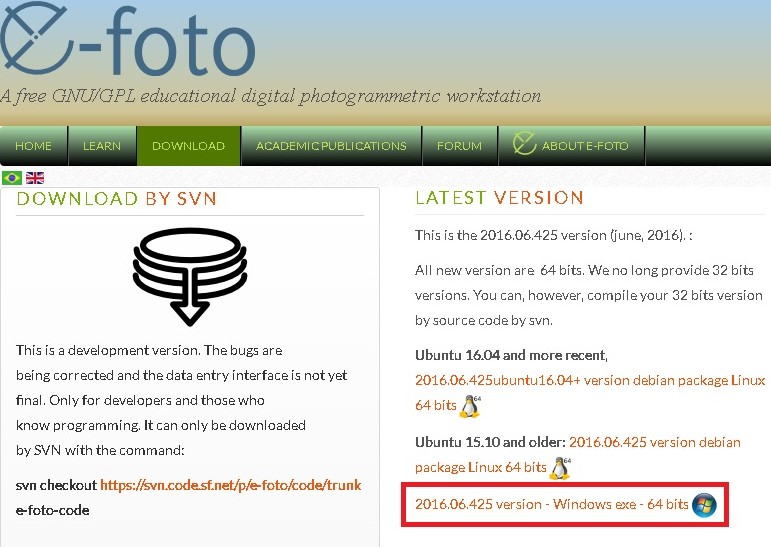
\includegraphics[width=10cm]{Figuras/downmsi.jpg} %use imagens com melhor resolução, em todo o projeto
	\caption{Realizando download do instalador do E-foto} \label{fig:downmsi}
\end{figure}

\subsubsection{Passo 2 - Realizar a instalação} %faltou a versão detalhada para Linux, com instruções na linha comando.
Normalmente o arquivo baixado vai para a pasta \textit{Downloads} do computador do usuário e para realizar a instalação basta dar um clique duplo nesse arquivo, clicar na opção \textit{Next}, ler e aceitar os termos do contrato, e clicar novamente em \textit{Next}.  No próximo passo o usuário deve escolher o caminho onde o E-foto será instalado. Depois o usuário deve clicar em \textit{Install} e a instalação será realizada automaticamente, conforme a Figura \ref{fig:installmsi}.
 
\begin{figure}[!ht]{17cm}
   \centering
   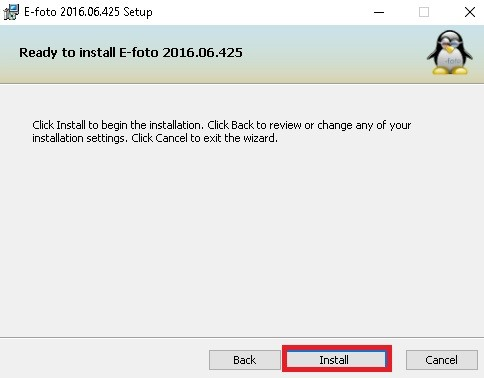
\includegraphics[width=10cm]{Figuras/installmsi.jpg}
   \caption{Instalando E-foto por meio do instalador} \label{fig:installmsi}
\end{figure}
  
\subsubsection{Passo 3 - Executar o programa E-foto}
Após a instalação terminar, basta manter a opção \textit{launch} E-foto e clicar na opção \textit{Finish}, como mostra a Figura \ref{fig:launch1} que o E-foto será executado, ou fechar o instalador e buscar o E-foto nos seus aplicativos instalados, conforme a Figura \ref{fig:launch2}. Neste formato o instalador do E-foto instalará tudo o que é necessário para o seu funcionamento, sem a necessidade de configurações adicionais.

\begin{figure}[!ht]{17cm}
	\centering
	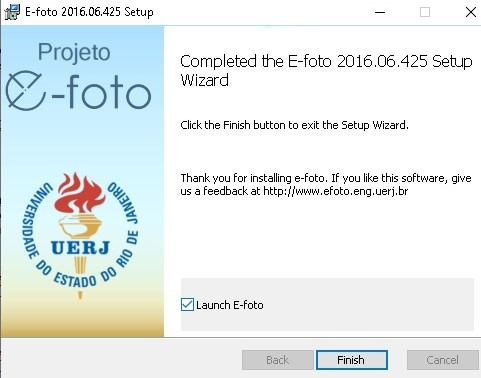
\includegraphics[width=10cm]{Figuras/launch1.jpg}
	\caption{Executando o E-foto pelo instalador} \label{fig:launch1}
\end{figure}

\begin{figure}[!ht]{17cm}
	\centering
	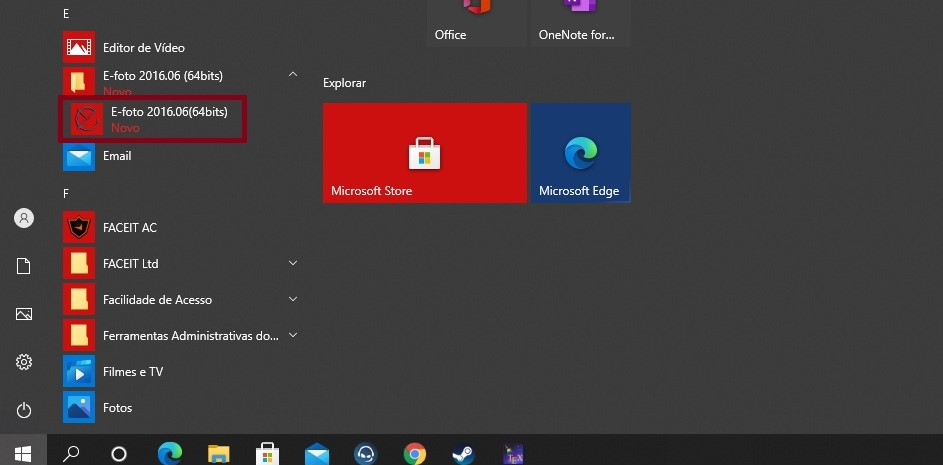
\includegraphics[width=12cm]{Figuras/launch2.jpg}
	\caption{Buscando E-foto nos aplicativos} \label{fig:launch2}
\end{figure}

\subsection{Compilação do E-foto a partir dos fontes}
\subsection{Em Sistemas Linux}

\subsubsection{Passo 1 - Baixar código fonte}
Primeiramente, para realizar a instalação do software E-foto, o usuário pode fazer o download do seu código fonte e para isso é necessário a instalação do \textbf{subversion}, se já não estiver instalado. Para tal, o usuário deve abrir o terminal do seu sistema Linux, que pode ser feito digitando terminal na barra de busca ao apertar a tecla do \textit{Windows} no seu teclado ou pelo atalho do teclado \texttt{ctrl + alt + T}. Com o terminal aberto, o usuário começará a instalação do SVN com os comandos: 
\begin{lstlisting}[language=bash]
	$ sudo apt update
	$ sudo apt install subversion
\end{lstlisting}

Com o SVN instalado e configurado, basta o usuário digitar no terminal o comando:
\begin{lstlisting}[language=bash]
 $ svn checkout https://svn.code.sf.net/p/e-foto/code
\end{lstlisting}

Com a utilização desse comando o download de todo o código fonte do software E-foto será feito automaticamente. 

Também é possível obter o código fonte por download direto... %completar aqui as instruções 
    
\subsubsection{Passo 2 - Instalar pacotes necessários à compilação}  
Após a realização do download do código fonte do E-foto, o usuário deve ficar atento aos pacotes necessários em seu ambiente para que o E-foto possa ser instalado e ter seu funcionamento sem erros. Para a instalação dos pacotes o usuário deve buscar abrir novamente o terminal. Os pacotes necessários para instalação do e-foto são: 
\begin{itemize}
   	\item libgdal.dev
   	\item build-essential
   	\item libfontconfig1
   	\item mesa-common-dev
   	\item libx11-xcb-dev
   	\item libglu1-mesa-dev
\end{itemize}
Cada pacote deve ser instalado com respectivamente com os seguintes comandos: %pode colocar tudo em 1 só comando	
\begin{lstlisting}[language=bash]
	$ sudo apt install libgdal-dev build-essential libfontconfig1 mesa-common-dev libx11-xcb-dev libglu1-mesa-dev
\end{lstlisting}				
	
O pacote \textit{libgdal.dev} contém as funcionalidades da GDAL, onde GDAL é uma biblioteca de tradução para formatos geoespaciais.%o que quer dizer tradução de formatos geospaciais?
 O pacote \textit{libfontconfig1} contém uma biblioteca projetada para achar fontes no sistema e selecioná-las de acordo com os requisitos especificados pelas aplicações, e o usuário deve instalar o driver \textbf{XCB} e o \textbf{OpenGl} por meio dos pacotes \textit{mesa-common-dev}, \textit{libx11-xcb-dev} e \textit{libglu1-mesa-dev}. %explicar para que serve cada pacote
    
\subsection{Passo 3 - Instalar os pacotes de instalação do Qt 5}   
A instalação do Qt 5 via terminal deve ser feita por meio dos seguintes pacotes:
\begin{itemize}
	\item qt5-default
	\item qt5-qmake
\end{itemize}   
Esses pacotes devem ser instalados por meio dos seguintes comandos do terminal:
\begin{lstlisting}[language=bash]
	$ sudo apt install qt5-default
	$ sudo apt install -y qt5-qmake
\end{lstlisting}	
    
Após esses procedimentos o usuário ja terá um ambiente de compilação pronto para a instalação do E-foto, assim como o plataforma em que o mesmo foi desenvolvido.
    
\subsection{Passo 4 - Compilar e executar o software E-foto}
Para compilar e executar o código do E-foto via terminal, após a realização de todos os passos necessários, o usuário deve utilizar os seguintes comandos no terminal:
\begin{lstlisting}[language=bash]
   	$ cd diretório/
   	$ qmake e-foto.pro
   	$ make
   	$ ./build/bin/e-foto
\end{lstlisting}
   
O comando \textit{cd diretório/} servirá para o usuário percorrer o caminho até o diretório onde está o arquivo \textbf{e-foto.pro} (atualmente \textit{code/branches/e-foto-trunk-candidate}), depois o \textit{qmake} e o \textit{make} irão realizar a compilação e gerar o executável do E-foto. Por fim o último comando irá executar o programa.

\subsection{Em Sistemas Windows}

\subsubsection{Passo 1 - Baixar código fonte}
Para começar a instalação do E-foto em sistemas \textit{Windows}, o usuário deve realizar o download do código fonte do E-foto e para isso o melhor caminho é utilizar o \textit{subversion}, que no \textit{Windows} pode ser feito através de um programa chamado \textbf{TortoiseSVN}, cuja versão usada para essa explicação foi a 1.14.0, e que pode ser baixado gratuitamente por esse link \url{https://tortoisesvn.net/downloads.html} na opção mostrada na Figura \ref{fig:tortoise}. Após a instalação do \textbf{TortoiseSVN}, o usuário deve buscar no programa a opção de SVN Checkout, que pode ser encontrada ao clicar o botão direito do mouse na área de trabalho conforme, é mostrado na figura \ref{fig:checkout} e no espaço para colar uma URL (primeira opção disponível) colocar \url{https://svn.code.sf.net/p/e-foto/code}, como é visto na Figura \ref{fig:url}. Isso deve gerar o download de todo o código fonte do E-foto.

Também existe a opção de baixar o código fonte diretamente do site...%completar
 
\begin{figure}[!ht]{17cm}
 	\centering
 	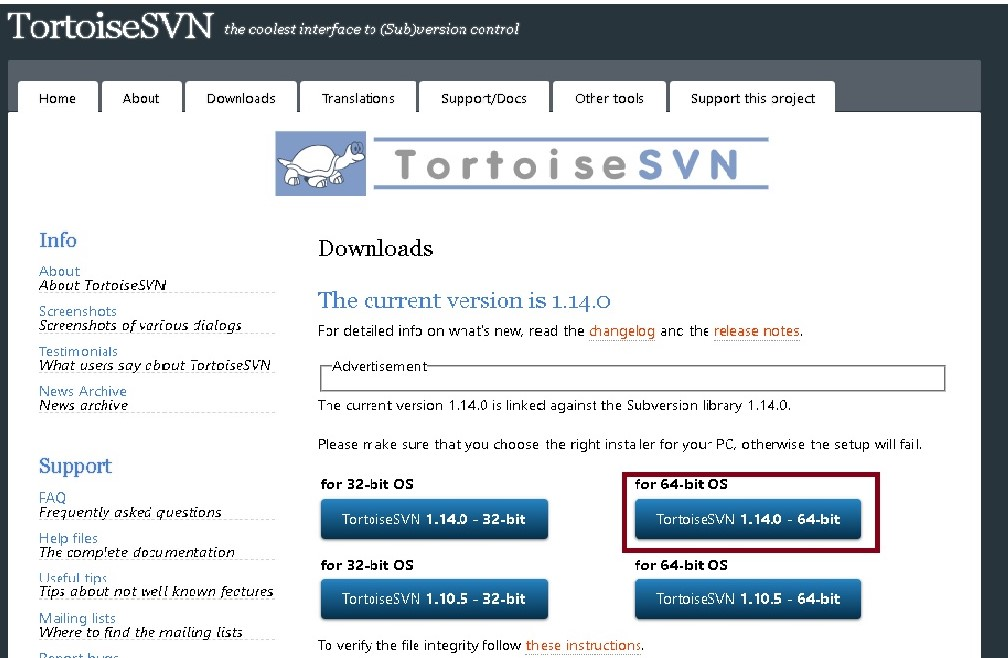
\includegraphics[width=12cm]{Figuras/tortoise.jpg}
 	\caption{Download do TortoiseSVN} \label{fig:tortoise}
\end{figure}

\begin{figure}[!ht]{17cm}
	\centering
	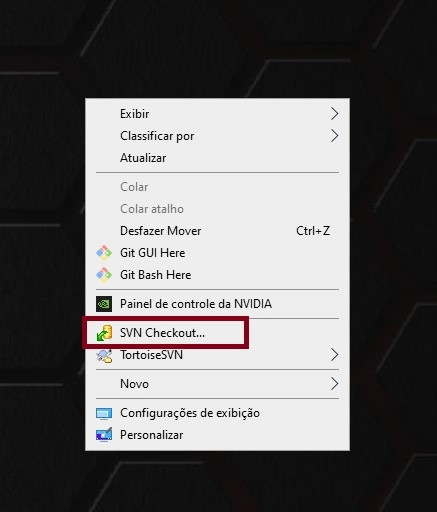
\includegraphics[width=10cm]{Figuras/checkout.jpg}
	\caption{Buscando a opção de checkout} \label{fig:checkout}
\end{figure}

\begin{figure}[!ht]{17cm}
	\centering
	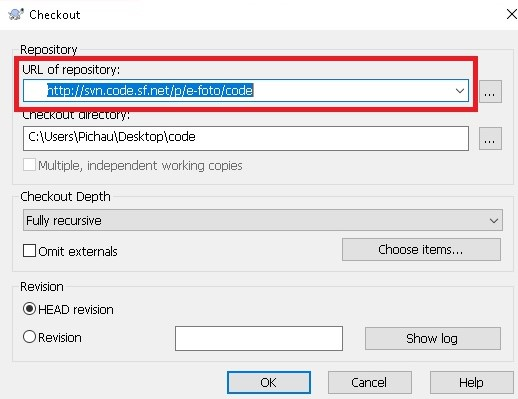
\includegraphics[width=12cm]{Figuras/url.jpg}
	\caption{Realizando o download com a URL} \label{fig:url}
\end{figure}
 
\subsubsection{Passo 2 - Download dos pacotes binários da Gdal no Windows} 
O próximo passo é o download dos pacotes binários da Gdal no \textit{Windows}. Isso pode ser realizado diretamente pelo link  \url{https://repo.msys2.org/distrib/x86\_64/msys2-x86\_64-20200720.exe}, que realizará o download do MSYS. Após a conclusão do download e da instalação do MSYS (que deve ser feita no drive C, que normalmente é o \textit{default}) o usuário deve executar \textbf{mSYS}, o que vai abrir o terminal do próprio MSYS que contém uma versão portada do gerenciador de pacotes \textit{Pacman} conforme pode ser visto na Figura \ref{fig:terminalgdal}. Nessa última versão do \textit{Pacman} deve ser digitado no terminal o comando:

\begin{lstlisting}[language=bash]
$ pacman -Syuu
\end{lstlisting}
 
\begin{figure}[!ht]{17cm}
 	\centering
 	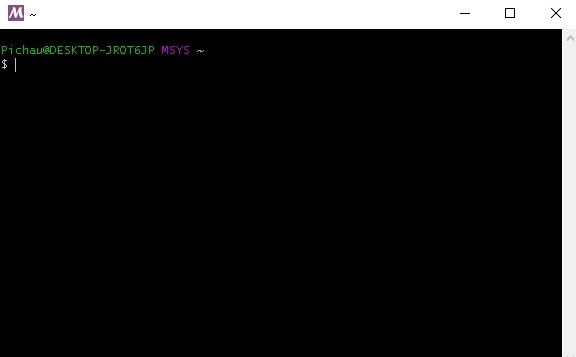
\includegraphics[width=12cm]{Figuras/terminalgdal.jpg}
 	\caption{Terminal MSYS} \label{fig:terminalgdal}
\end{figure}
 

Esse comando irá gerar uma série de instruções a serem seguidas até que o usuário possa repetir o comando e receber a mensagem de que nada necessita ser atualizado. Com o ambiente atualizado, o usuário deve digitar o seguinte comando:
\begin{lstlisting}[language=bash]
 	$ pacman -S mingw64/mingw-w64-x86\_64-gdal
 	$ gdalinfo --version
\end{lstlisting}

Esses comandos realizarão finalmente o download e instalação dos pacotes binários da GDAL e dirão qual versão que foi instalado, respectivamente. 
 
\subsubsection{Passo 3 - Baixar e configurar o Qt 5 e o Qt Creator}
Nessa etapa o usuário pode realizar o download do \textbf{Qt 5} e do \textbf{Qtcreator} no website do Qt\footnote{\url{https://www.qt.io/download}}, como mostrado na Figura \ref{fig:downqt}, deixando claro que na parte da instalação deve ser escolhido para instalar apenas as opções do \textit{mingw} 64-bits, e o Qt 5 referente a esse sistema (Figura \ref{fig:qtinstallconfig}). Com os arquivos do código fonte do E-foto disponíveis, o usuário deve procurar no caminho \textit{e-foto-code/branches/e-foto-trunk-candidate} por um arquivo chamado \textbf{e-foto.pro}, como mostrado na Figura \ref{fig:openpro}. Quando abrir o projeto no \textit{Qtcreator} será necessário configurar o que deverá ser usado, começando pela escolha do kit que será usado, que deve ser o mesmo escolhido na instalação do Qt 5, ou seja, o \textit{mingw} 64-bits e a versão do Qt referente a esse sistema, como mostra a Figura \ref{fig:qtkit}. Após o projeto estar aberto, o usuário deve ir na guia \textit{project} e desmarcar a opção \textit{shadow build}, e depois procurar e clicar na aba \textbf{build} a opção \textit{build E-foto}. Quando acabar a compilação é só clicar na opção \textbf{Run}, que também pode ser encontrado na aba \textit{build}, e o E-foto vai abrir pronto para o uso como está assinalado na Figura \ref{fig:projectbuild}.
\begin{figure}[!ht]{17cm}
  	\centering
 	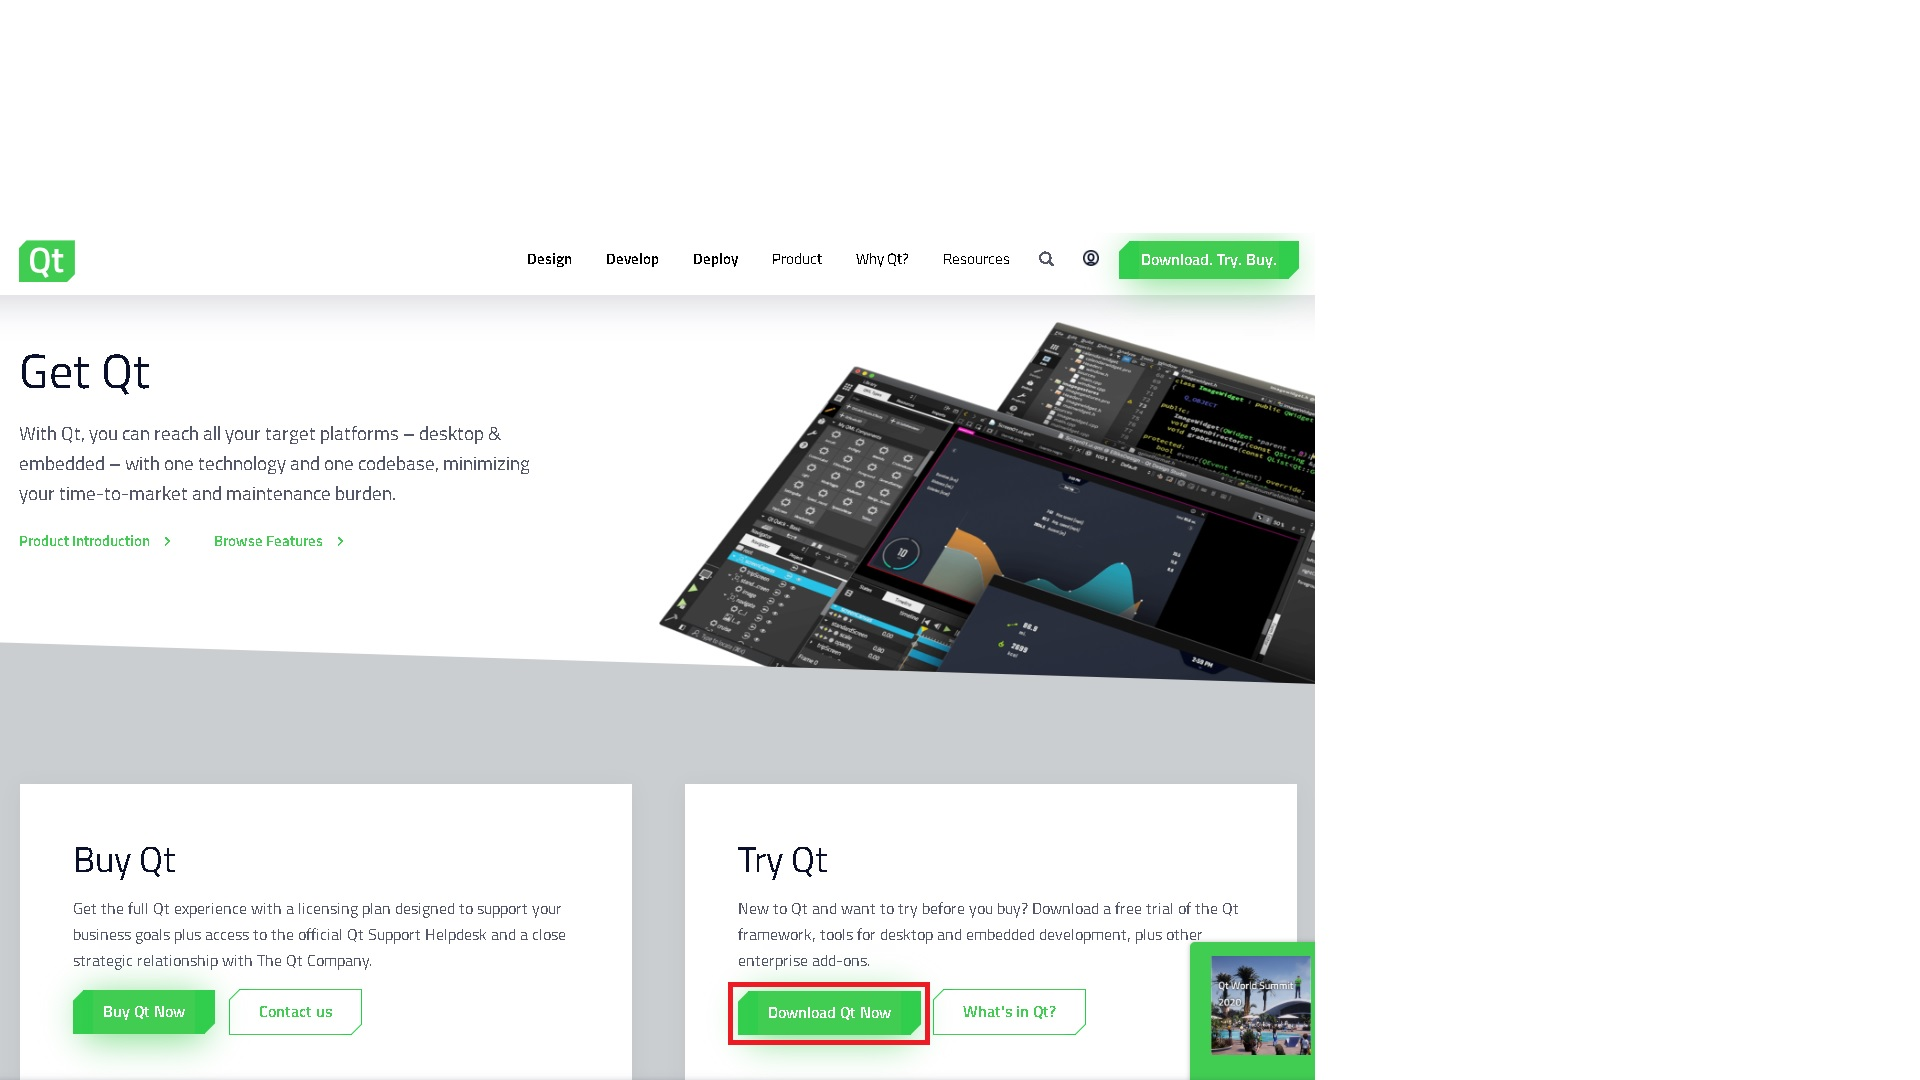
\includegraphics[width=12cm]{Figuras/downqt.jpg}
 	\caption{Download do Qt 5 pelo website} \label{fig:downqt}
\end{figure}

\begin{figure}[!ht]{17cm}
 	\centering
	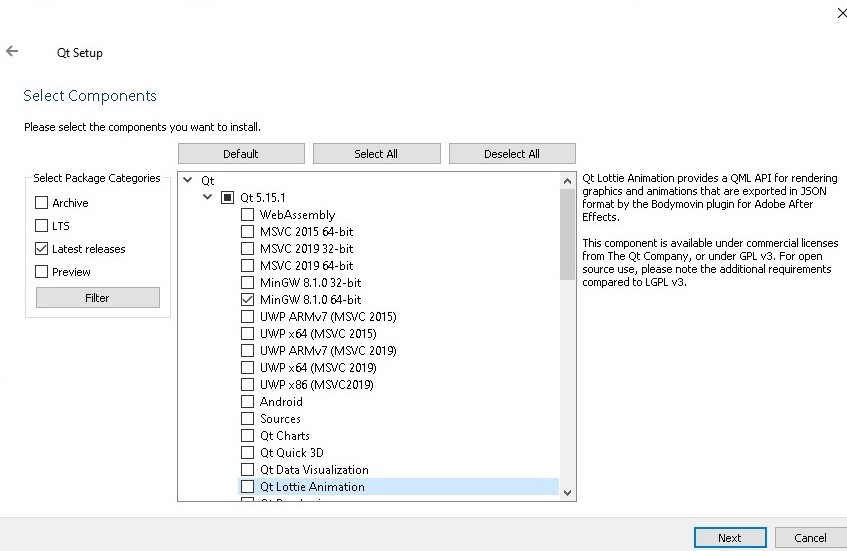
\includegraphics[width=12cm]{Figuras/qtinstallconfig.jpg}
	\caption{Configuração da instalação do Qt 5} \label{fig:qtinstallconfig}
\end{figure}

\begin{figure}[!ht]{17cm}
 	\centering
	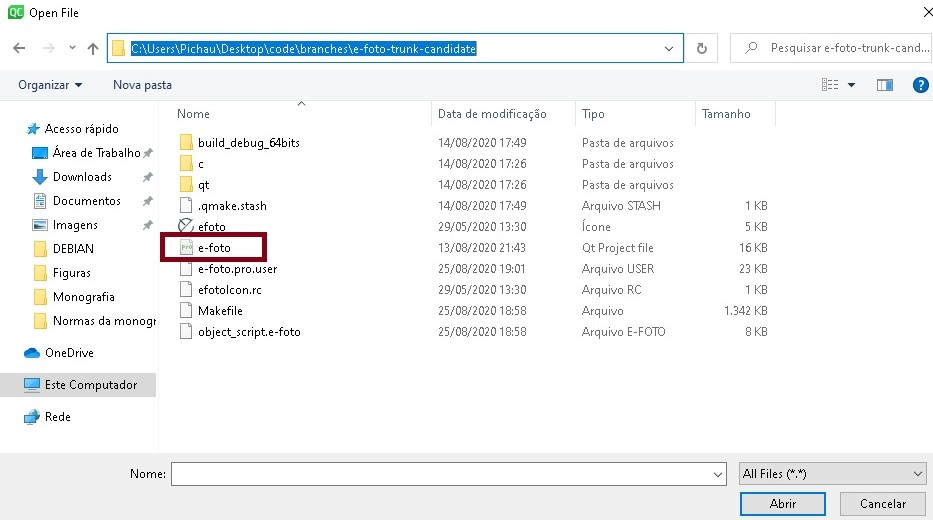
\includegraphics[width=15cm]{Figuras/openpro.jpg}
	\caption{Caminho do arquivo do projeto E-foto} \label{fig:openpro}
\end{figure}

\begin{figure}[!ht]{17cm}
 	\centering
	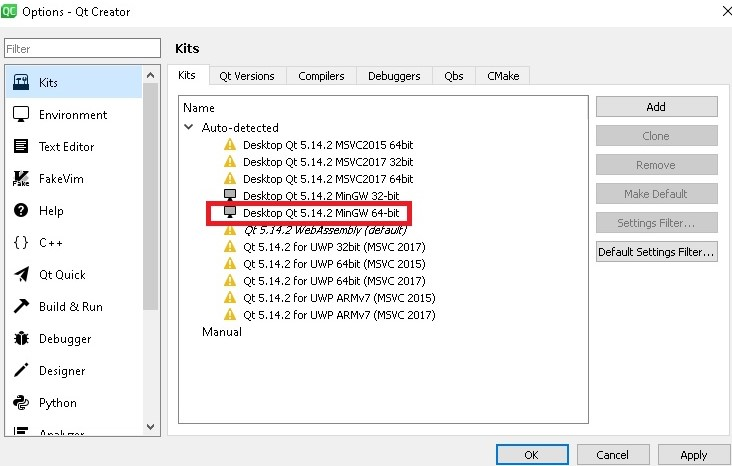
\includegraphics[width=15cm]{Figuras/qtkit.jpg}
	\caption{Configuração do kit} \label{fig:qtkit}
\end{figure}

\begin{figure}[!ht]{17cm}
 	\centering
	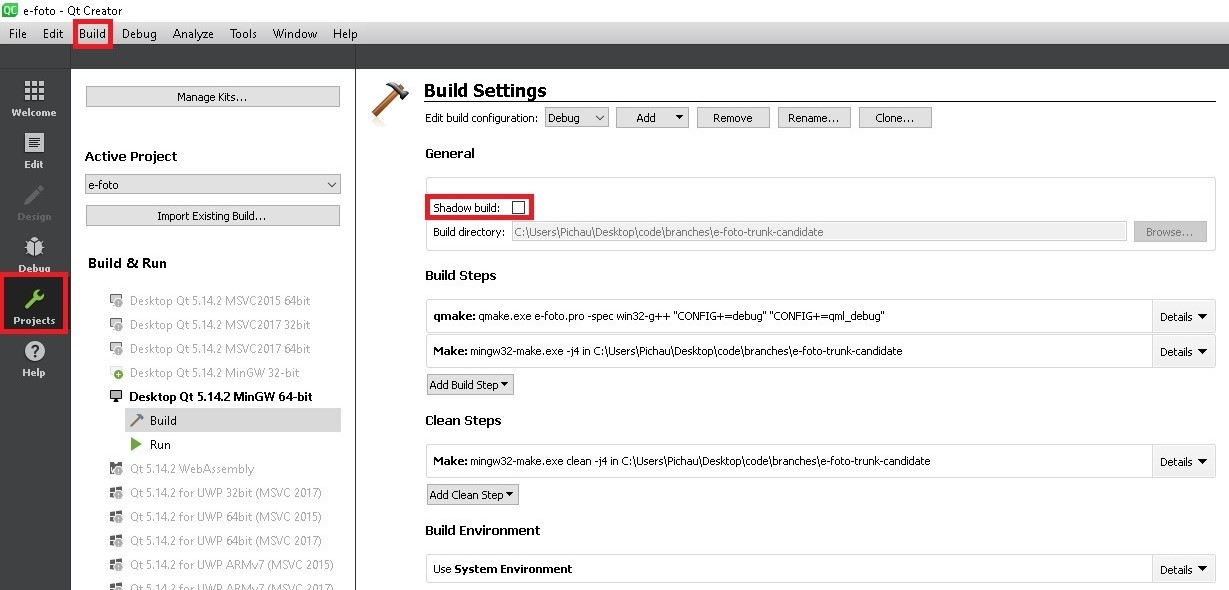
\includegraphics[width=15cm]{Figuras/projectbuild.jpg}
	\caption{Locais buscados para a compilação} \label{fig:projectbuild}
\end{figure}
 
	%================================================================
\chapter{Debian-GIS}
%================================================================
\section{O que é o Debian-GIS}

O \textbf{Debian-GIS} é um \textit{Debian Pure Blend}, o que significa ser uma parte do Debian nos quais seus pacotes estão agrupados e disponíveis para um determinado grupo de usuários que possuem necessidades especiais, tornando desnecessário o acesso a todos os pacotes Debian disponíveis. O \textit{Debian-GIS} tem como objetivo atender os usuários interessados em um Sistema de Informação Geográfica, ou seja, visa satisfazer as necessidades de usuários que trabalham com mapas, sensoriamento remoto e observação da Terra e dispõe de uma lista de programas GIS selecionados para o Debian.

A equipe \textit{Debian-GIS} também atua em conjunto para ajudar a manter o software GIS atual em derivados Debian, como \textbf{UbuntuGIS}, que reempacota os pacotes do Debian-GIS nas diferentes distribuições do Ubuntu, e \textbf{OSGeo-Live} fornece aplicativos pré-configurados para uma variedade de casos de uso geoespacial, incluindo armazenamento, publicação, visualização, análise e manipulação de dados. Ele também contém conjuntos de dados de amostra e documentação.

De acordo com o site \url{https://debian-gis-team.pages.debian.net/policy/packaging.html} \cite{bib:gis}:

\begin{quote}
	``O Debian GIS se orgulha de que derivados estão lucrando com o trabalho dentro do Debian e está tentando estabelecer conexões fortes com esses derivados. Com o UbuntuGIS, a conexão é tão forte que um fluxo de trabalho comum foi criado, onde os desenvolvedores do UbuntuGIS estão injetando seu pacote diretamente no sistema de controle de versão do Debian-GIS. Para ter certeza de que não haverá conflitos com as revisões do Debian, deve-se prestar atenção à numeração das revisões.''
\end{quote}

\subsection{Tasks}

De acordo com o site \url{https://debian-gis-team.pages.debian.net/policy/tasks.html} \cite{bib:gis}:

\begin{quote}
	``O Debian GIS Debian Pure Blend é organizado por tasks, que agrupam pacotes em torno de temas amplos como serviços web e estação de trabalho. As tasks listam programas que já estão empacotados no Debian assim como pacotes em preparação. Os arquivos de tasks não são hospedados nos repositórios Debian-GIS, mas no repositório Debian Blends, em uma área de trabalho de computador normal, o usuário provavelmente desejará instalar pelo menos a task da estação de trabalho que contém os aplicativos GIS mais usados. Os meta-pacotes do Debian GIS Blend podem ser instalados em uma instalação normal do Debian. Como isso pode ser feito depende de qual versão do Debian você está executando.''  
\end{quote}

Estes são os metapacotes citados acima que podem ser instalados usando o comando apt-get install (nome do metapacote):

\begin{itemize}
	\item gis-data - dados Debian GIS
	\item gis-gps - programas relacionados a GPS
	\item gis-osm - Programas relacionados ao OpenStreetMap
	\item gis-remotesensing - Sensoriamento remoto e observação da Terra
	\item gis-statistics - Estatísticas com dados geográficos
	\item gis-web - Apresentar informações geográficas via web mapserver
	\item gis-workstation - estação de trabalho de Sistemas de Informação Geográfica (GIS)
	\item gis-devel - pacotes de desenvolvimento GIS

\end{itemize}

\section{Sistemas Debian}
% falta revisar
O sistema Debian ou Debian GNU/Linux é um sistema operacional que faz parte do projeto Debian, que é uma organização de pessoas com interesse em comum de criar um sistema operacional livre. Nesse projeto os membros são voluntários, e o sistema operacional Debian, que é um conjunto de programas básicos e utilitários que fazem o computador funcionar, pode ser obtido gratuitamente na web.

O sistema Debian é muito conhecido devido ao seu poderoso sistema de gerenciamento de pacotes (APT, Advanced Packaging Tool ou Ferramenta de Empacotamento Avançada) que permite a instalação de novos pacotes, além da atualização e remoção dos pacotes antigos de forma limpa e relativamente fácil. O Debian possui acesso a repositórios online com uma quantidade enorme de pacotes, sendo oficialmente apenas softwares livres. Softwares não-livres também podem ser baixados e instalados caso seja necessário.

De acordo com o próprio site oficial do Debian o \url{www.debian.org}, o Debian é uma organização totalmente voluntária dedicada a desenvolver software livre e promover os ideais da comunidade de Software Livre. O projeto Debian se iniciou em 1993, quando Ian Murdock ofereceu um convite livre a desenvolvedores de software livre para contribuir com uma distribuição completa e coerente baseada no kernel do Linux relativamente novo. O nome “Debian” vem da junção do nome do principal fundador, Ian, com o de sua esposa, Debra. Os Desenvolvedores Debian estão envolvidos em uma variedades de atividades, incluindo Web e FTP, administração do site, design gráfico, análise legal de licenças de software, escrevendo documentação, e é claro, mantendo pacotes de softwares.

\subsection{Vantagens da utilização do Debian}
A página oficial \url{www.debian.org/intro/why\_debian.pt.html} lista o motivo de escolher o \textit{Debian} para utilizar em uma máquina e entre suas principais vantagens estão:

\begin{itemize}
	\item Velocidade na resolução de dúvidas em sua lista de discussão;
	\item O sistema é mantido por seus próprios usuários;
	\item Existem muitas empresas e pessoas que usam o Debian, o que pode ser visto através do site \url{www.debian.org/users};
	\item O Dpkg é um dos melhores sistema de empacotamento atualmente, cansativos testes são feitos para incluir softwares novos aos sistema Debian stable;
	\item Instalação melhorada periodicamente, já que antes a dificuldade de instalação era um problema bem comentado pelos interessados em migrar para o debian;
	\item São mais de 59.000 programas diferentes;
	\item Atualização do Sistema simplificado com o APT;
	\item Suporte para múltiplas arquiteturas (alpha, amd64, armel, hppa, i386, ia64, mips, mipsel, powerpc, s390, e sparc);
	\item Estabilidade, Leve e Rápido, Drivers escritos pelos usuários, sem dependência dos fabricantes.
\end{itemize}

Mas como nada é perfeito o Debian também tem alguns pontos de reclamação que ainda estão sendo otimizados, que são:

\begin{itemize}
	\item Nem todo hardware é suportado;
	\item O Debian é difícil de configurar;
	\item Falta de software comercial popular.

\end{itemize}

\subsection{Derivados do Debian}

De acordo com o site \url{www.debian.org/derivatives/index.pt.html}: 

\begin{quote}
	``Existem várias distribuições baseadas no Debian. Algumas pessoas podem querer dar uma olhada nessas distribuições além dos lançamentos oficiais do Debian. Um derivado do Debian é uma distribuição baseada no trabalho realizado no Debian, mas com sua própria identidade, objetivos e público-alvo, e é criado por uma entidade que é independente do Debian. Os derivados modificam o Debian para atingir os objetivos que eles mesmos estabeleceram. O Debian dá boas-vindas e encoraja organizações que desejam desenvolver novas distribuições baseadas no Debian. No espírito do contrato social do Debian, é esperado que os derivados contribuam com seu trabalho para o Debian e os projetos dos autores originais, para que todos possam se beneficiar de suas melhorias.''
\end{quote}

O direcionamento do público de certo nicho para o derivado Debian que contém usuários que partilham de objetivos semelhantes, ajuda a manter a satisfação do usuário com o Debian como um todo, já que seu acesso a recursos será direcionado a realização das tarefas de seu nicho com mais facilidade e sem a necessidade de ter que conhecer e dominar todos os recursos do Debian. E dado esse aumento na satisfação do publico de diferentes nichos, é de se esperar que a comunidade Debian cresça como um todo.

\section{Requisitos para um software ser aceito no Debian-GIS}

No geral para um pacote ser aceito no \textit{Debian-GIS} as regras são basicamente as mesmas para que o pacote seja aceito no Debian, pois é aconselhável seguir o caminho normal para a aceitação de pacotes Debian em pacotes \textit{Debian-Gis}. Porém existem algumas edições no arquivo \textit{control} do repositório Debian do software empacotado que devem ser realizadas e que são específicas para o Debian-Gis de acordo com a Política oficial Debian-GIS que pode ser encontrada através do link \url{https://debian-gis-team.pages.debian.net/policy/policy.html}.

\subsection{Mudanças no diretório Debian/control}
De acordo com a Política Oficial do Debian-GIS, as seguintes mudanças devem ser feitas obrigatoriamente para que o pacote seja aceito:
\begin{verbatim}
Section (Seção): Deve ser “science” para o pacote de origem.
Priority (Prioridade): Deve ser “optional” a menos que proibido pela
política Debian.
Maintainer (Mantenedor): O mantenedor deve ser Debian GIS Project
<pkg-grass-devel@lists.alioth.debian.org>. O usuário pode se
inscrever também nesta lista caso queira participar.
Uploaders: O usuário deve se increver como um uploader quando
tiver um interesse significativo em um pacote.
\end{verbatim}

\subsection{Busca por um sponsor}

Para quem não é um desenvolvedor oficial do Debian, para que o pacote seja posto no Debian é necessária a busca por um sponsor que revisará esse pacote e realizará a operação de \textit{upload}. Existem vários \textit{Debian Developers} na equipe \textit{Debian-GIS}, infelizmente eles estão muito ocupados e podem não responder aos pedidos de patrocínio enviados para a Lista de Discussão dos Desenvolvedores \textit{Debian-GIS}. Portanto, é recomendado seguir o processo normal do Debian e enviar um relatório de bug de Solicitação de Patrocínio (RFS). O site \textit{Debian Mentors} é o melhor lugar para enviar seu pacote para atrair patrocinadores, o site também fornece um modelo para o seu relatório de bug RFS.

O relatório de bug RFS também deve ser copiado para a lista de discussão dos desenvolvedores GIS do Debian. A melhor maneira de fazer isso é usar o cabeçalho\textit{ X-Debbugs-CC} no relatório de bug. Adicione \textit{X-Debbugs-CC: pkg-grass-devel@lists.alioth.debian.org} ao cabeçalho de e-mail da mensagem ou use a opção \textbf{s} no utilitário reportbug.
	%================================================================
\chapter{Pacote Debian do E-foto}
%================================================================
\section{Requisitos do E-foto}

Aqui será explicada a criação do pacote Debian do E-foto de acordo com as regras da Debian Policy \cite{bib:Ian}, cujo material de auxílio usado foi manual de empacotamento de Debian \cite{bib:Lucas}, o guia para novos mantenedores do Debian \cite{bib:Josip} e o guia rápido do empacotamento no Debian \cite{bib:Filho2020}.  

\subsection{Pacotes para a criação de um pacote de acordo com a política do Debian}

Primeiramente estão listados nos comandos abaixo os pacotes necessários para a criação de um pacote Debian, de acordo com a política do Debian, que deve ser criado num ambiente \textit{Debian unstable}. % o que ṕe debian unstable?

\begin{lstlisting}[language=bash]
	$ apt update
	$ apt install install autopkgtest blhc locales devscripts dh-make dput-ng git-buildpackage mc quilt spell tardiff tree
\end{lstlisting}

\begin{description}
	\item[Pacote autopkgtest] - enumera os testes do pacote e especifica suas dependências e requisitos.
	\item[Pacote blhc] - resolve possíveis problemas de hardening %para que serve isso?
	 (processo de proteção) na compilação de pacotes que são escritos em C ou C++.
	\item[Pacote locales] - contém ferramentas para gerar definições de localidade de arquivos de origem, uma vez que quando um ambiente Debian unstable é criado, configurações de localidade terão de ser feitas pois são reiniciadas. %explicar melhor
	\item[Pacote devscripts] - contém diversos scripts que facilitam a vida do empacotador, pois seguem a política do Debian.
	\item[Pacote dh-make] - realiza a automatização de diversas etapas do empacotamento, além de gerar o diretório debian parcialmente preenchido de acordo com a política do Debian mais atual, evitando assim uma série de erros que podem ser cometidos no processo de empacotamento de algum software.
	\item[Pacote dput-ng] - é uma ferramenta de upload de pacotes para o Debian que fornece uma interface fácil de usar para instalações de hospedagem de arquivos de pacotes Debian. Ele permite que qualquer um que trabalhe com pacotes Debian carregue seu trabalho para um serviço remoto, incluindo ftp-master do Debian, mentors.debian.net, Launchpad ou outras facilidades de hospedagem de pacotes para mantenedores de pacotes Debian.
	\item[Pacote git-buildpackage] - ferramenta que facilita o manuseio de pacotes Debian em repositórios Git, uma vez que o git é uma forma de controle de versão tanto do software fornecido pelo upstream tanto como do próprio processo de empacotamento.%é necessário no caso od efoto, já que usamos svn?
	\item[Pacote mc] - é um gerenciador de arquivos de tela inteira em modo texto. Ele usa uma interface de dois painéis e um subshell para execução de comandos. Inclui um editor interno com destaque de sintaxe e um visualizador interno com suporte para arquivos binários.
	\item[Pacote quilt] - é um gerenciador de patches, % explicar o que é um patch
	 acompanhando as mudanças que cada um deles faz. E funciona os organizando logicamente como uma pilha e você pode aplicá-los, desaplicá-los e atualizá-los facilmente viajando para a pilha. Esse pacote só é necessário caso exista algum patch de mudança no empacotamento.
	\item[Pacote spell] - é um programa de verificação ortográfica que imprime cada palavra incorreta em uma linha própria, muito bom para garantir que nenhum arquivo do pacote conterá erros ortográficos, é de muita importância que o empacotador utilize o mesmo após a finalização de cada arquivo para realizar a verificação, pois encontrará dificuldades de ter seu pacote aceito pelo Debian, caso tenha erros de ortografia.
	\item[Pacote tardiff] - compara o conteúdo de dois tarballs % sempre que introduzir um termo, explicá-lo
	 e relata quaisquer diferenças encontradas entre eles. Seu uso é principalmente para gerentes de lançamento que podem usá-lo como uma ferramenta de controle de qualidade para garantir que nenhum arquivo tenha sido deixado de lado acidentalmente ou adicionado por engano. TarDiff suporta tarballs compactados, estatísticas de diferenças e supressão de mudanças GNU autotool. Esse pacote é muito usado pois como pode ser visto no manual do desenvolvedor do Debian, o código fonte do upstream geralmente vem no formato .tar.gz.
	\item[Pacote tree] - é um comando recursivo de listagem de diretórios que produz uma listagem de arquivos em formato de árvore. Muito usado para realizar a verificação de como ficou o empacotamento, se cada arquivo e diretório estão localizados em seu devido lugar.
	\item[Pacote lintian] - é um sistema que disseca os pacotes Debian e relata bugs e violações de políticas. Ele contém verificações automatizadas para muitos aspectos da política do Debian, bem como algumas verificações para erros comuns. Ele usa um diretório de arquivo, denominado “laboratório”, no qual armazena informações sobre os pacotes que examina. Ele pode manter essas informações entre várias chamadas para evitar a repetição de operações caras de coleta de dados. Isso torna possível verificar o repositório Debian completo em busca de bugs, em um tempo razoável. Este pacote é útil para todas as pessoas que desejam verificar os pacotes Debian quanto à conformidade com a política Debian. Cada mantenedor do Debian deve verificar os pacotes com esta ferramenta antes de enviá-los.
\end{description}
 
\section{Criação do Pacote Debian do E-foto}
%mostrar um passo a passo

\subsection{Verificação de Intenção de Empacotar}

Antes de realizar o empacotamento de qualquer software para o Debian deve ser feita a verificação se não existe esse mesmo software já empacotado ou se algum outro programador já declarou a intenção de empacotá-lo. Para isso é necessário acessar o site \url{https://wnpp.debian.net/} ou o site \url{https://bugs.debian.org/cgi-bin/pkgreport.cgi?pkg=wnpp;dist=unstable} e procurar o nome do software que será empacotado, pois pacotes duplicados não são aceitos pelo Debian. Ao fazer isso com o E-foto foi encontrado o bug de intenção de empacotar \url{https://bugs.debian.org/cgi-bin/bugreport.cgi?bug=899283}, mas essa tentativa não obteve sucesso pois na época o E-foto ainda estava em Qt 4. Agora com o empacotamento da sua versão em Qt 5 deverá ser criado um outro bug para que o novo pacote seja aceito. %colocar a data da tentativa

\subsection{Processo de criação de uma jaula de ambiente Debian unstable}

O primeiro passo para a criação de um pacote de acordo com a política do Debian é a obtenção de uma ambiente \textit{Debian unstable}, já que todo empacotamento deve ser feito em um ambiente \textit{Debian unstable} (com exceções de modificações ou correções em pacotes já publicados no \textit{Debian stable}), pois o pacote vai entrar no \textit{Debian unstable}, depois passar para \textit{experimental} até poder ser classificado e utilizado no \textit{stable}, mas para a realização desse empacotamento o empacotador não precisará usar uma versão \textit{unstable} do Debian caso não seja sua preferência, será suficiente a criação de apenas um ambiente chamado também de \textit{jaula-sid} que é justamente um diretório dentro do \textit{Debian stable} em que o desenvolvedor estará confinado e que dentro dele estará o \textit{Debian unstable} e essa jaula pode ser criada a partir dos comandos: %Parágrafo está mjuito longo, com sentenças muito longas. Dividir parágrafo em mais frases. colocando pontos e não apenas vírgulas. Explicar esse termo jaula.

\begin{lstlisting}[language=bash]
	$ apt update
	$ mkdir /jaula-sid
	$ debootstrap sid /jaula-sid/ftp.br.debian.org/debian
	$ chroot /jaula-sid/
	$ echo proc /proc proc defaults 0 0 >> etc/ fstab
	$ wget http://bit.ly/bash-rc-txt
	$ apt install autopkgtest blhc locales devscripts dh-make dput-ng git-buildpackage mc quilt spell tardiff tree lintian
	$ apt-get clean
	$ dpkg-configure locales tzdata
\end{lstlisting}

\begin{description}

	\item[Comando mkdir /jaula-sid] - cria um diretório na raiz com o nome de jaula-sid. O nome \textbf{sid} vem do nome do Debian \textit{unstable}.
	\item[Comando debootstrap sid /jaula-sid/\textit{ftp.br.debian.org/debian}] - realiza o download e a instalação de um ambiente Debian unstable no diretório jaula-sid a partir do link indicado para download da imagem.
	\item[Comando chroot /jaula-sid/] - altera a raiz para o diretório jaula-sid, tornando-o isolado ou ``enjaulado'' de forma em que ele não conseguirá acessar nada fora dele mesmo. Com isso, o empacotador ficará a partir daqui utilizando só a versão \textit{unstable} do Debian. É desse método que foi inspirado o nome jaula para o diretório de empacotamento.
	\item[Comando echo proc /proc proc defaults 0 0 >> etc/ fstab] - cria um dispositivo proc (é um diretório especial onde ficam todas as informações de depuração do \textit{kernel}, também se encontram algumas configurações que habilitam e desabilitam o suporte à alguma coisa no \textit{kernel}) que vai garantir o funcionamento correto da jaula.
	\item[Comando wget \textit{http://bit.ly/bash-rc-txt}] - realiza o download de um arquivo de texto que contém uma série de comandos de configuração e ele deve ser colocado no \textit{/etc/bash.bashrc} pois esse diretório é lido sempre que ocorre a troca de ambiente para o Debian unstable.
	\item[Comando cat bash-rc-txt >> /etc/bash.bashrc] - coloca o arquivo no diretório correto como explicado acima.

\end{description}

O conteúdo do bash-rc-txt é o seguinte:
\begin{verbatim}
alias ls='ls --color=auto' 
alias tree='tree -aC' 
alias debuildsa='dpkg-buildpackage -sa -ksua_chave_gpg' 
alias uscan-check='uscan --verbose --report' 
alias debcheckout='debcheckout -a' 
export DEBFULLNAME="seu_nome_completo_sem_acentos/cedilha" 
export DEBEMAIL="seu_e-mail" export EDITOR=mcedit 
export LANG=C.UTF-8 export LANGUAGE=C.UTF-8 
export LC_ALL=C.UTF-8 
export QUILT_PATCHES=debian/patches 
export PS1='JAULA-SID-\u@\h:\w\$ ' 
mount /proc 
\end{verbatim}

Agora é o momento de realizar a instalação de alguns pacotes essenciais para o funcionamento correto da jaula. É importante frisar que a jaula deve ser mantida o mais limpa possível, ou seja, só pacotes realmente essenciais devem ser instalados, pois isso pode afetar na hora da construção e compilação do pacote. Esse procedimento é o descrito na subseção acima. O próximo passo de configuração do ambiente de trabalho é configurar o \textit{locales} (que define quais idiomas serão usados e qual o idioma padrão do ambiente de trabalho, geralmente pt\_BR.UTF-8) e o fuso horário (São Paulo, cidade que está no centro do fuso) por meio do comando
\begin{verbatim}
$ dpkg-configure locales tzdata
\end{verbatim}
Agora deve ser feita a configuração do \textit{lintian}, e para realizar essa configuração deve ser criado o arquivo \textit{/root/.lintianrc} com as seguintes linhas: 

\begin{verbatim}
display-info = yes 
pedantic = yes 
display-experimental = yes 
color = auto.
\end{verbatim}

Após isso é necessário usar o comando
\begin{lstlisting}[language=bash]
$ apt-get clean
\end{lstlisting}
para eliminar arquivos desnecessários e poupar espaço para iniciar o empacotamento.

Agora, a próxima etapa deve ser assinar o pacote com a chave GPG do empacotador, caso seja da escolha dele, da seguinte maneira: fora da jaula, exporte as suas chaves GPG (privada e pública) com os comandos: %como criar uma chave gpg, caso não possua?

\begin{lstlisting}[language=bash]
	$ gpg -a --export nr_da_chave > nr_da_chave.pub 
	$ gpg -a --export-secret-keys nr_da_chave > nr_da_chave.key
\end{lstlisting} 
%nr é número? não está explícito.

Mova os arquivos para dentro da jaula \textit{unstable}% como eu faço isso na linha de comando?
, volte para a jaula com o comando
\begin{lstlisting}[language=bash]
$ chroot /jaula-sid/
\end{lstlisting}
, importe as chaves e remova os arquivos. Para importar use os seguintes comandos: % e para remover?

\begin{lstlisting}[language=bash]
	$ gpg --list-keys 
	$ echo "pinentry-mode loopback" >> ~/.gnupg/gpg.conf 
	$ gpg --import chave.key chave.pub 
\end{lstlisting}

Agora para habilitar a chave para assinatura de pacotes o empacotador deve editar o arquivo \textit{/etc/devscripts.conf} e inserir o número completo da chave GPG na linha \textit{DEBSIGN\_KEYID}, descomentando-a. Com isso, finalmente a jaula de trabalho está pronta e configurada para começar o empacotamento.

\subsection{Começando o processo de empacotamento}

%nomes de pacote só podem conter letras minúsculas, números e símbolos sendo que no mínimo dois algarismos.
Primeiramente o empacotador deve instalar o programa e testá-lo para ver se ele realmente funciona e se vale a pena empacotá-lo.

Após feito isso, para começar realmente o empacotamento, é preferível a criação dentro da jaula de trabalho de um diretório com o nome genérico do pacote (por exemplo \textit{pkgnome-do-programa}) com o comando: %porque não usar aqui o nome já do efoto?

\begin{lstlisting}[language=bash]
	$ mkdir pkgnome-do-programa 
\end{lstlisting} 

Dentro desse diretório a primeira etapa é obter o código fonte do \textit{upstream} que de acordo com o manual de desenvolvedores deve estar preferencialmente no formato \textit{.tar.gz} (tarball) e descompactá-lo. A política geral de software do \textit{Debian} prevê que para realizar o empacotamento, o diretório raiz deve ser nomeado da seguinte forma: \textbf{nomedoprograma-numerodeversão}. Logo após isso, o empacotador deve preferencialmente verificar o licenciamento do programa e isso pode ser feito de duas formas distintas: uma é por meio do comando: \textit{lincensecheck} * % tudo que for comando coloque em linha separada.
(que dará como resultado a licença de cada arquivo dentro do código fonte fornecido pelo upstream) ou através do comando\textit{ egrep -sriA25 '(public dom|copyright)' | less} (que toda vez em que as expressões \textit{public dom} ou \textit{copyright} forem citadas nos arquivos-fontes as 25 linhas posteriores serão mostradas, assim mostrando o que o autor do código explicitou sobre a licença). Esse procedimento deve ser feito com calma e de maneira bem minuciosa para novos pacotes pois o Debian não aceita nenhum mínimo detalhe que comprometa o fato de o código ser livre.

O próximo passo será um dos mais importantes pois é a "debianização" do código fonte (a criação do diretório Debian dentro do código junto com seus arquivos necessários de acordo com a política do Debian) e isso é feito através do comando:

\begin{lstlisting}[language=bash]
	$ dh_make -f ../.tar.gz -c <licença> 
\end{lstlisting} 

\subsection{Modificando o conteúdo do diretório Debian do pacote}

Os primeiros arquivos do diretório Debian a ser modificados são os que são obrigatórios para o empacotamento:\textbf{ Changelog, Control, Copyright e Rules.} Devido a utilização do pacote \textit{dh-make}, esses arquivos já virão previamente preenchidos com algumas informações que deverão ser modificadas de acordo com o conteúdo do software que está sendo empacotado.

Começando pela edição do \textit{debian/changelog} que no caso de ser a primeira vez em que o software está sendo empacotado, é só alterar o modelo para se adequar ao seu pacote com informações básicas (alterar de \textit{unstable} para \textit{experimental} em caso de ser o primeiro empacotamento do programa, por exemplo), mas futuramente toda modificação no pacote que vai gerar uma revisão pelo Debian deve ser documentada nesse arquivo. 

O segundo a ser editado será o \textit{debian/control} que também já vem com o formato preenchido sendo necessário só alterar os valores de acordo com o programa, e esses valores são divididos em dois parágrafos, o superior trata do código fonte e o inferior trata do binário que será gerado.

Sobre os campos do fonte (parágrafo superior):
\begin{verbatim}
Source: nome do programa.
Section: é o nome da seção em que se enquadra a funcionalidade do programa que
será empacotado, essas funções e suas descrições podem ser vistas no site 
https://packages.debian.org/unstable/.
Priority: prioridade em que o programa deve ser instalado no Debian, serve
para controlar quais pacotes são instalados junto com o Debian em determinadas 
configurações e essa prioridade deve ser determinada apenas pela funcionalidade
que o programa fornece ao usuário.
Maintainer: nome do mantenedor do pacote, geralmente junto com e-mail.
Build-depends: são os pacotes que tem que ser obrigatoriamente instalados para
que instalação do programa, como os pacotes são para desenvolvimento, geralmente
eles têm -dev no final. O pacote que necessariamente o empacotador está usando
é o debhelper-compat (=13).
Standards-version: A versão mais recente dos padrões (o manual de política e
textos associados) com os quais o pacote está em conformidade. 
Homepage: É a página da internet onde o código fonte pode ser obtido.
\end{verbatim}

Sobre o binário (parágrafo inferior):
\begin{verbatim}
Package: nome do pacote que será gerado.
Architecture: aqui deve ser especificado pra qual tipo de arquitetura o 
empacotador quer que seu pacote seja gerado. Geralmente são any 
(programas em linguagem compilada) ou all (programas em linguagem 
interpretada), mas caso o programa só funcione em uma arquitetura específica,
ela deve ser especificada aqui nesse campo.
Depends: são auxiliares que na construção do binário busca dependências
do código que não foram especificadas. 
Description: é dividida em duas partes, a descrição curta e a descrição longa.
A descrição curta deve ser rápida e objetiva com as funcionalidades do programa.
Já a longa geralmente é copiada da descrição do autor que é dada na homepage do
upstream porém deve ser formatada de acordo com a politica Debian, toda linha 
tem que ser indentada com um espaço em branco, o comprimento de cada linha é de
no máximo 80, caso exista uma linha em branco entre parágrafos ela deve ser
preenchida com um ponto final e geralmente é preferível que esse texto seja
escrito de maneira impessoal.
\end{verbatim}

Existem outros campos possíveis mas esses listados são os obrigatórios e necessários, esses outros campos podem ser vistos nesse site \url{https://www.debian.org/doc/debian-policy/ch-controlfields.html}

O próximo a ser preenchido é o \textit{debian/copyright} com os seguintes campos:
\begin{verbatim}
Format: já vem preenchido com o formato que está sendo seguido para a realização
do  copyright.
Upstream-Name: Nome do programa.
Upstream-Contact: Geralmente é colocado aqui o endereço da página do upstream
usada para o envio de bugs.
Source: Homepage do usptream.
Cada arquivo que tiver uma licença diferente deve ser especificado com esses
3 campos:
Files: nome do arquivo.
Copyright: autor e data.
License: nome da licença.
Geralmente todo código tem uma especificação de lincença  para o código fonte
e outra para o diretório debian no caso de o autor do programa e o autor do
empacotamento sejam diferentes. Ou pode ser colocados o mesmo para que os 
códigos possam ser misturados.
License: Explicação completa feita sobre o que diz a licença. 
\end{verbatim}

Agora será editado o campo \textit{debian/rules}. Este campo já vem comentado com algumas sugestões de preenchimento. Devem ser deixadas as seguintes linhas:
\begin{verbatim}
#!/usr/bin/make -f
#export DH\_VERBOSE = 1
#export DEB\_BUILD\_MAINT\_OPTIONS = hardening=+all
#export DEB\_CFLAGS\_MAINT\_APPEND = -Wall -pedantic
#export DEB\_LDFLAGS\_MAINT\_APPEND = -Wl, --as-needed

%:
dh $@

\end{verbatim}
O restante deve ser apagado e cada linha de comentário deixada só pode ser descomentada em caso de necessidades especiais do programa que serão sanadas com as mesmas. O arquivo \textit{rules} é o \textit{makefile} dentro do diretório Debian do pacote e é nele que devem ser especificados quaisquer peculiaridades da construção do programa, para que o pacote possa ser montado de maneira bem-feita. Ao final do empacotamento, após a realização dos testes do pacote, essa linhas de comentários que não tiveram utilidade devem ser apagadas.

Por último será preenchido o \textit{debian/watch} com as seguintes informações:
\begin{verbatim}
Version: a versão do watch que está sendo usada (deve ser usada sempre
a mais atual).
As próximas linhas devem ser preenchidas com links onde devem ser 
procuradas possíveis atualizações feitas pelo upstream no código fonte.
Geralmente são preenchidos com links de sites usados para o controle de 
versão de programas ou códigos como o Github ou Sourceforge.
É importante deixar claro que pra realizar o empacotamento o empacotador
deve apagar todo lixo, comentário e coisas desnecessárias. O pacote deve
ser o mais limpo e leve possível.
\end{verbatim}

\subsection{Construção do pacote}

Após todas as etapas citadas anteriormente, é hora de usar o comando \textit{debuild} no diretório raiz e esperar a compilação do programa e criação do pacote. Quando acabar muito possivelmente aparecerão alguns erros \textit{lintian} que deverão ser corrigidos para que o pacote esteja de acordo com a política do Debian, a maneira mais fácil de corrigir esses erros \textit{lintians} é acessando o site \url{https://lintian.debian.org/tags.html} e procurar a explicação do erro que está acontecendo e como resolvê-lo. Quando o seu pacote estiver sem erros \textit{lintians}, ou só com \textit{lintians} que não são solucionáveis (não podendo ser \textit{lintians} de erro ou algo relacionado a obrigações do pacote ou empacotador) chegou a hora de realizar as checagens finais e começar a buscar as maneiras de subir esse pacote para o Debian.

\subsection{Testes finais do pacote}

Logo após a construção do pacote e resolução dos erros \textit{lintians}, o empacotador deve realizar mais alguns testes antes de enviar seu pacote para o Debian, primeiramente ele deve passar o comando \textit{spell} em todos os arquivos que ele mesmo criou do diretório Debian, depois ele deve usar o comando \textit{tree nomedopacote} dentro do diretório Debian do pacote para verificar como foi feita a construção do mesmo, ou seja, se cada arquivo foi para o lugar em que deveria após o empacotamento. E nessa verificação é importante perceber se o \textit{dh\_compress} fez seu papel corretamente, já que ele é uma ferramenta do \textit{debhelper} que comprime todo arquivo com tamanho maior que 4k (com a exceção de arquivos \textit{copyright}, \textit{.html} e outros arquivos web, arquivos de imagens, e arquivos que aparentam já estarem comprimidos com base nas suas extensões), essa compressão de arquivos é feita de acordo com a política do Debian e o \textit{dh\_compress} é chamado automaticamente junto com o comando \textit{debuild} usado para a construção do pacote.

Após essa etapa o empacotador deve verificar novamente todos os arquivos do diretório Debian e usar o comando \textit{debuild} duas vezes para ter certeza de que não ocorrerá nenhum novo erro na construção do pacote. A ultima etapa é usar o \textit{cowbuilder} para testar a construção do pacote em uma jaula \textit{unstable} limpa e isso é feito através dos seguintes comandos:

\begin{lstlisting}[language=bash]
	$ cowbuilder create
	$ cowbuilder update
	$cowbuilder build arquivo.dsc
\end{lstlisting} 

Esses comandos vão criar o ambiente \textit{Debian unstable} limpo, atualizar o mesmo e testar a construção do pacote nesse ambiente respectivamente. Esse teste é de total importância pois durante o processo de empacotamento pode ser gerada uma poluição na jaula que acabará influenciando no resultado final, e com esse teste em um ambiente limpo ocorre uma simulação de como o pacote será construído e testado nos servidores do Debian quando for feito seu \textit{upload}.
	%================================================================
\chapter{Resultados}
%================================================================

\section{Testes}

\subsection{Ubuntu}
Para começar os testes no \textit{Ubuntu}, foi usada a versão 20.04 do mesmo onde primeiramente foi testado o pacote gerado através do empacotamento feito na \textit{Jaula-SID} que, como explicado anteriormente, cria um ambiente \textit{Debian Unstable} dentro do próprio \textit{Ubuntu}, gerando assim um pacote que contém dependências mais atualizadas do que as disponíveis no \textit{Ubuntu}. Este empacotamento segue as politicas do Debian e também se baseia parcialmente no \textbf{Manual de Empacotamento de Debian} que pode ser obtido em sua versão traduzida para o português através do endereço: \url{https://www.debian.org/doc/manuals/packaging-tutorial/packaging-tutorial.pt.pdf}.
 
Devido a esse problema de compatibilidade os primeiro testes acabaram gerando erro durante a instalação do pacote, e esses erros não eram contornáveis, uma vez que esses pacotes cujo o pacote E-foto tinha como dependência não tinham essas versões disponíveis de maneira alguma no \textit{Ubuntu 20.04}. 

Após algum tempo de estudo e pesquisas foi decidido o teste através da realização de um empacotamento diretamente no Ubuntu 20.04, sem a utilização da \textit{Jaula-SID} ou qualquer outro tipo de ambiente \textit{Debian Unstable}. Seguindo novamente de maneira parcial o \textbf{Manual de Empacotamento de Debian} e também o passo-a-passo que foi descrito aqui anteriormente, ocorreu a criação de um novo pacote com sucesso, porém durante a compilação do mesmo um novo erro \textit{lintian} apareceu, que trazia a mensagem retratando que o sistema operacional em que um novo pacote deve ser criado é o \textit{Debian Unstable} e que a versão do sistema operacional usado estava entrando em conflito com essa política.

Mas mesmo com essa nova mensagem de advertência, a compilação ocorreu com sucesso assim como a geração do pacote e após isso, foi só instalar o pacote através do comando:

\begin{lstlisting}[language=bash]
	$ sudo dpkg -i nome_do_pacote 
\end{lstlisting}

como pode ser visto na figura \ref{fig:ubuntu_insta}, buscar o caminho do diretório onde o \textit{E-foto} foi instalado através do terminal e utilizar o comando:

\begin{lstlisting}[language=bash]
	$ ./efoto
\end{lstlisting}

no diretório onde fica o executável, geralmente \textit{usr/bin} como é mostrado na figura \ref{fig:ubuntu_exec}.

\begin{figure}[!ht]{17cm}
	\centering
	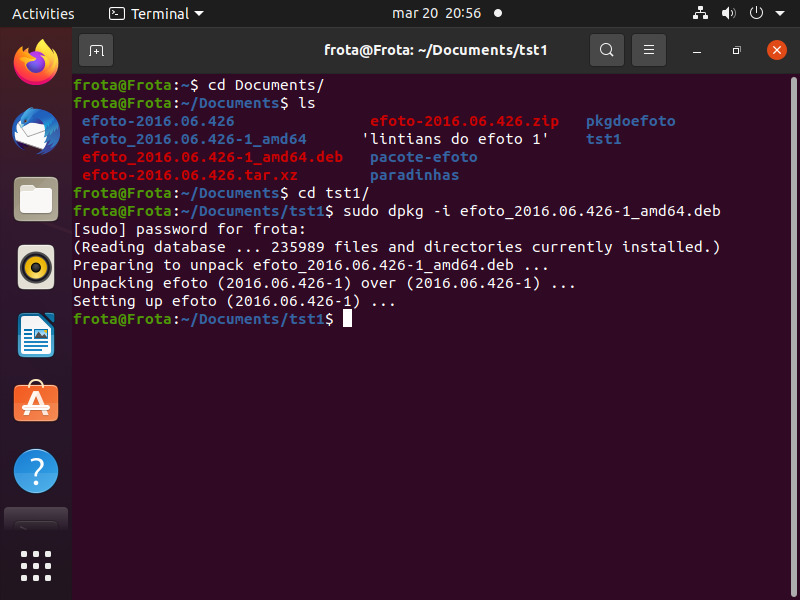
\includegraphics[width=15cm]{Figuras/ubuntu_insta.jpg}
	\caption{Instalação do pacote E-foto no Ubuntu} \label{fig:ubuntu_insta}
\end{figure}

\begin{figure}[!ht]{17cm}
	\centering
	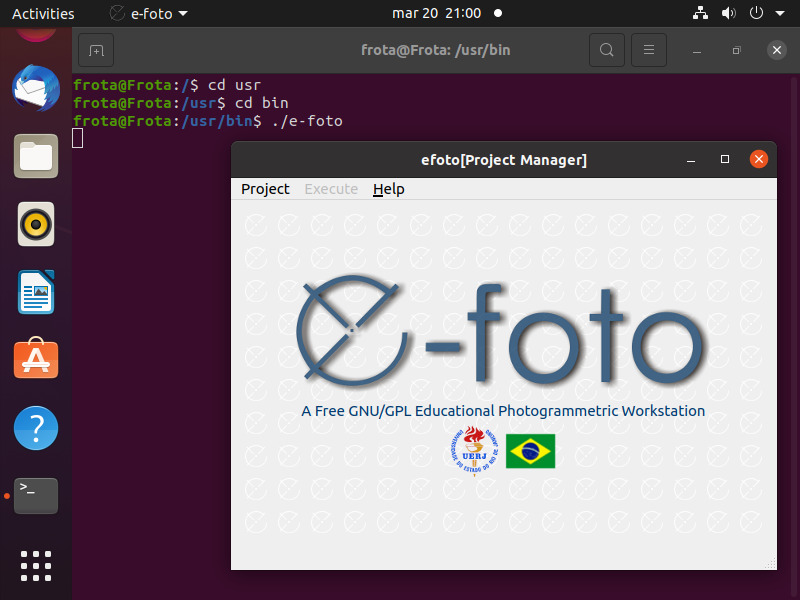
\includegraphics[width=15cm]{Figuras/ubuntu_exec.jpg}
	\caption{Funcionamento do executável gerado pelo pacote E-foto no Ubuntu} \label{fig:ubuntu_exec}
\end{figure}


\subsection{Debian Unstable}

Para começar o teste do funcionamento do pacote do software E-foto no sistema operacional \textit{Debian} em sua versão instável completa, que é o ambiente correto para a realização destes teste devido á ser neste ambiente que o próprio Debian realizará a primeira etapa de testes quando o pacote for finalizado e disponibilizado, é necessária a obtenção dessa versão instável do Debian, e para isso são necessários alguns passos, uma vez que essa versão não é disponibilizada diretamente para download no site do Debian. O método escolhido para instalação da versão instável do Debian foi através da alteração do arquivo \textbf{source.list} através do terminal de comando na versão do \textit{Debian testing} mais atual. 

O primeiro passo é a realização do download da versão mais atual do \textit{Debian testing} mais atual, que pode ser obtida através do endereço \url{https://www.debian.org/devel/debian-installer} e que poderá ser instalada em uma máquina própria ou em uma máquina virtual. Após a instalação do sistema operacional \textit{Debian Testing}, a próxima etapa é a edição do arquivo \textbf{source.list} através da linha de comando no caminho \textit{/etc/apt/source.list} substituindo o seu conteúdo com pelo seguinte:

\begin{verbatim}
deb http://ftp.br.debian.org/debian/ unstable main contrib non-free	
deb-src http://ftp.br.debian.org/debian/ unstable main contrib non-free
\end{verbatim}

Depois é preciso salvar e sair. Novamente no terminal de comando deve ser usado o comando:

\begin{lstlisting}[language=bash]
	$ sudo apt update
\end{lstlisting}

para que todos as listas de pacotes possam ser atualizadas, obtendo assim as versões mais recentes de cada pacote disponível no local especificado pelo \textbf{source.list} e depois o ultimo passo é o comando:

\begin{lstlisting}[language=bash]
	$ sudo apt upgrade
\end{lstlisting}

que instalará as versões mais recentes de todos os pacotes que já estão instalados no sistema baseados no local especificado pelo arquivo \textbf{source.list}. Com o fim da realização destes passos, a versão instável do Debian estará disponível para uso e consequentemente para a realização do teste do pacote.

Para testar o funcionamento do pacote, é preciso ir através do terminal de comando até o local onde está o arquivo .deb do E-foto e utilizar o comando:

\begin{lstlisting}[language=bash]
	$ sudo dpkg -i nome_do_pacote
\end{lstlisting}

que a instalação ocorrerá automaticamente como é demonstrado na figura \ref{fig:debian_insta}, porém para que isso aconteça o pacote \textbf{libgdal.dev} deve estar instalado previamente, após a instalação ser concluída, basta ir até o local onde foi instalado o E-foto, buscar o seu arquivo executável, que geralmente é instalado no \textit{usr/bin}, e usar o comando:

\begin{lstlisting}[language=bash]
	$ ./efoto
\end{lstlisting}

que o programa será executado perfeitamente como pode ser visto na figura \ref{fig:debian_exec}.

\begin{figure}[!ht]{17cm}
	\centering
	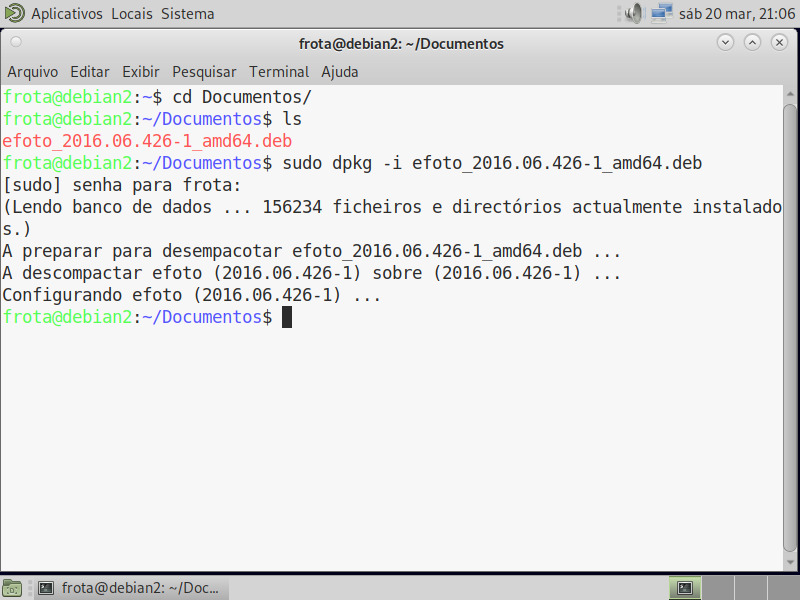
\includegraphics[width=15cm]{Figuras/debian_insta.jpg}
	\caption{Instalação do pacote E-foto no Debian} \label{fig:debian_insta}
\end{figure}

\begin{figure}[!ht]{17cm}
	\centering
	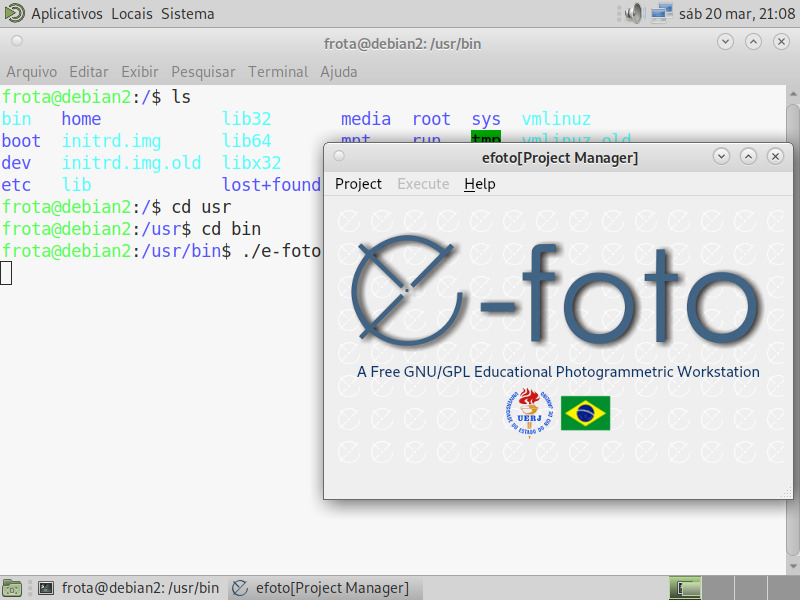
\includegraphics[width=15cm]{Figuras/debian_exec.jpg}
	\caption{Funcionamento do executável gerado pelo pacote E-foto no Debian} \label{fig:debian_exec}
\end{figure}
	%================================================================
\chapter{Conclusão}

O trabalho realizado permitiu que fosse percebida a grande diferença entre as formas de instalação do software E-foto em diferentes sistemas operacionais evidenciando assim os benefícios trazidos a partir do empacotamento do mesmo. Porém ainda assim foi deixado explicado em forma de tutorias de linguagem bem simples as maneiras corretas de se obter e instalar o E-foto nos sistemas operacionais mais usados.

Foi visto claramente que obter o pacote do E-foto simplifica bastante sua instalação se comparada com as outras formas de instalação mostradas e torná-lo um pacote aceito pelo \textit{Debian-GIS} facilitará a propagação dos benefícios do software e de suas funcionalidades para o nicho correto que se interessará por elas. Aumentando assim o grupo que se interessará pela utilização do E-foto. 

Outro ponto benéfico da realização do trabalho foi a expansão do conhecimento para além das salas de aulas e das disciplinas do curso de computação, já que foi necessário um certo aprendizado sobre o tema da cartografia uma vez que é sobre esse tema que o E-foto trata.

Por último foi constatada a importância do trabalho que vem sendo realizado pelo grupo que mantém o E-foto, pois gera um oportunidade gigantesca de aprendizado de alunos de áreas distintas, bem como o trabalho em equipe de aprimoramento do software e o acesso gratuito a uma estação fotogramétrica digital.     

	
	
	%\index{Introdução!Capítulo}.
	
	%XXXXXXXXXXXXXXXXXXXXXXXXXXXXXXXXXXXXXXXXXXXXXXXXXXXXXXXXXXXXXXXX
	% ELEMENTOS POS-TEXTUAIS
	%XXXXXXXXXXXXXXXXXXXXXXXXXXXXXXXXXXXXXXXXXXXXXXXXXXXXXXXXXXXXXXXX
	\backmatter % inicia a área dos elementos pós-textuais
	%XXXXXXXXXXXXXXXXXXXXXXXXXXXXXXXXXXXXXXXXXXXXXXXXXXXXXXXXXXXXXXXX
	
	%===========================================================
	% Referencias via BibTeX
	%===========================================================
	
	\citeoption{abnt-options4}
	\bibliography{abnt-options4,bibliografia}
	
	%===========================================================
	\postextualchapter*{Glossário} % elemento opcional
	%===========================================================
	
	\definicao{termo 1}{significado}
	\definicao{termo 2}{significado}
	\definicao{termo 3}{significado}
	
	%XXXXXXXXXXXXXXXXXXXXXXXXXXXXXXXXXXXXXXXXXXXXXXXXXXXXXXXXXXX
	% Apêndices (opcionais)
	%XXXXXXXXXXXXXXXXXXXXXXXXXXXXXXXXXXXXXXXXXXXXXXXXXXXXXXXXXXX
	\appendix % inicia os apêndices
	%XXXXXXXXXXXXXXXXXXXXXXXXXXXXXXXXXXXXXXXXXXXXXXXXXXXXXXXXXXX
	
	%===========================================================
	
	%===========================================================
	\include{capAntigoProjeto}
	\include{capProfile}
	\include{capFicha}
	
	%===========================================================
	%===========================================================
	%XXXXXXXXXXXXXXXXXXXXXXXXXXXXXXXXXXXXXXXXXXXXXXXXXXXXXXXXXXX
	% Anexos (opcionais)
	%XXXXXXXXXXXXXXXXXXXXXXXXXXXXXXXXXXXXXXXXXXXXXXXXXXXXXXXXXXX
	\annex % inicia os anexos
	%XXXXXXXXXXXXXXXXXXXXXXXXXXXXXXXXXXXXXXXXXXXXXXXXXXXXXXXXXXX
	
	%===========================================================
	\postextualchapter{Primeiro anexo}
	%===========================================================
	
	% ----------------------------------------------------------
	\section{Primeira seção}
	% ----------------------------------------------------------
	
	Texto da primeira seção.
	
	% ----------------------------------------------------------
	\subsection{Primeira subseção}
	% ----------------------------------------------------------
	
	Texto da primeira subseção.
	
	% ----------------------------------------------------------
	\subsubsection{Primeira subsubseção}
	% ----------------------------------------------------------
	
	Texto da primeira subsubseção.
	
	%===========================================================
	\postextualchapter{Segundo anexo}
	%===========================================================
	
	% ----------------------------------------------------------
	\section{Primeira seção}
	% ----------------------------------------------------------
	
	Texto da primeira seção.
	
	% ----------------------------------------------------------
	\subsection{Primeira subseção}
	% ----------------------------------------------------------
	
	Texto da primeira subseção.
	
	% ----------------------------------------------------------
	\subsubsection{Primeira subsubseção}
	% ----------------------------------------------------------
	
	Texto da primeira subsubseção.
	
	%/\/\/\/\/\/\/\/\/\/\/\/\/\/\/\/\/\/\/\/\/\/\/\/\/\/\/\/\/\/
\end{document}
%/\/\/\/\/\/\/\/\/\/\/\/\/\/\/\/\/\/\/\/\/\/\/\/\/\/\/\/\/\/